\documentclass[journal]{vgtc}                % final (journal style)
%\documentclass[review,journal]{vgtc}         % review (journal style)
%\documentclass[widereview]{vgtc}             % wide-spaced review
%\documentclass[preprint,journal]{vgtc}       % preprint (journal style)


\pagenumbering{arabic}

% Section Numbering, remove this in submission 
% \setcounter{tocdepth}{4}
% \setcounter{secnumdepth}{4}

\makeatletter
\def\@copyrightspace{\relax}
\makeatother


% Load basic packages
\usepackage{balance}  % to better equalize the last page
\usepackage{graphics} % for EPS, load graphicx instead 
\usepackage[T1]{fontenc}
\usepackage{txfonts}
\usepackage{mathptmx}
\usepackage[pdftex]{hyperref}
\usepackage{color}
\usepackage{xcolor}
\usepackage{booktabs}
\usepackage{textcomp}
\usepackage{xspace}
\usepackage{setspace}
\usepackage[textsize=tiny]{todonotes}
% Some optional stuff you might like/need.
\usepackage{microtype} % Improved Tracking and Kerning
% \usepackage[all]{hypcap}  % Fixes bug in hyperref caption linking
\usepackage{ccicons}  % Cite your images correctly!
% \usepackage[utf8]{inputenc} % for a UTF8 editor only
\usepackage{verbatim}
\usepackage{relsize}
\usepackage{etoolbox}
\usepackage{lipsum}   % for filler text
\usepackage{setspace} % for \onehalfspacing and \singlespacing macros
\usepackage[normalem]{ulem}
\usepackage[sort,nocompress]{cite}
\usepackage{xcolor}
\def\plaintitle{Accelerating Scientific Data Exploration \\ via Visual Query Systems}

\def\plainauthor{Doris Jung-Lin Lee, John Lee, Tarique Siddiqui, Jaewoo Kim, Karrie Karahalios, Aditya Parameswaran}
\def\emptyauthor{} 
\def\plainkeywords{Data visualization, exploratory data analysis, visual query, scientific data.}
\def\plaingeneralterms{Documentation, Standardization}

% llt: Define a global style for URLs, rather that the default one
\makeatletter
\def\url@leostyle{%
  \@ifundefined{selectfont}{
    \def\UrlFont{\sf}
  }{
    \def\UrlFont{\small\bf\ttfamily}
  }}
\makeatother

\newenvironment{denselist}{
    \begin{list}{\small{$\bullet$}}%
    {\setlength{\itemsep}{0ex} \setlength{\topsep}{0ex}
    \setlength{\parsep}{0pt} \setlength{\itemindent}{0pt}
    \setlength{\leftmargin}{1.5em}
    \setlength{\partopsep}{0pt}}}%
    {\end{list}}

\newcommand{\squishlist}{
   \begin{list}{$\bullet$}
    { \setlength{\itemsep}{0pt}
      \setlength{\parsep}{2pt}
      \setlength{\topsep}{0pt}
      \setlength{\partopsep}{0pt}
      \leftmargin=25pt
\rightmargin=0pt
\labelsep=5pt
\labelwidth=10pt
\itemindent=0pt
\listparindent=0pt
\itemsep=\parsep
    }
}
\newcommand{\squishend}{\end{list}}

% use extensively to toggle between paper and TR
\newcommand{\eat}[1]{}
% \newcommand{\papertext}[1]{{\leavevmode\color{blue}{#1}}}
% \newcommand{\techreport}[1]{{\leavevmode\color{red}{#1}}}
\newcommand{\papertext}[1]{#1}
\newcommand{\techreport}[1]{#1} % show up in tvcg
\newcommand{\notvcgTR}[1]{} % things to remove from tvcg but include in TR
\newcommand{\nonannon}[1]{#1}
\newcommand{\annon}[1]{}
\newcommand{\boldpara}[1]{\textbf{\paragraph{#1}}}
% de-facto paragraph format
\newcommand{\stitle}[1]{\noindent\textbf{#1}}
% \newcommand{\tvcg}[1]{{\leavevmode\color{blue}{#1}}}
\newcommand{\tvcg}[1]{#1}
\newcommand{\cut}[1]{{\leavevmode\color{lightgray}{#1}}}
\newcommand{\ccut}[1]{} %confirmed cut

\urlstyle{leo}

% To make various LaTeX processors do the right thing with page size.
\def\pprw{8.5in}
\def\pprh{11in}
\special{papersize=\pprw,\pprh}
\setlength{\paperwidth}{\pprw}
\setlength{\paperheight}{\pprh}
\setlength{\pdfpagewidth}{\pprw}
\setlength{\pdfpageheight}{\pprh}

% Make sure hyperref comes last of your loaded packages, to give it a
% fighting chance of not being over-written, since its job is to
% redefine many LaTeX commands.
\definecolor{linkColor}{RGB}{6,125,233}
\hypersetup{%
  pdftitle={\plaintitle},
% Use \plainauthor for final version.
%  pdfauthor={\plainauthor},
  pdfauthor={\emptyauthor},
  pdfkeywords={\plainkeywords},
  bookmarksnumbered,
  pdfstartview={FitH},
  colorlinks,
  citecolor=black,
  filecolor=black,
  linkcolor=black,
  urlcolor=linkColor,
  breaklinks=true}

% create a shortcut to typeset table headings
% \newcommand\tabhead[1]{\small\textbf{#1}}
\newcommand{\zv}{\textit{zenvisage}\xspace}
\newcommand{\astro}{\textit{astro}\xspace}
\newcommand{\bio}{\textit{genetics}\xspace}
\newcommand{\matsci}{\textit{matsci}\xspace}

\newcommand{\agp}[1]{\textcolor{teal}{Aditya: #1}}
\newcommand{\kk}[1]{\textcolor{red}{Karrie: #1}} 
\newcommand{\dor}[1]{\textcolor{violet}{Doris: #1}} 
% Get rid of gaps between sections, subsections and subsubsections
% \usepackage{titlesec}
% \titlespacing*{\section}
% {0pt}{0pt}{0pt}
% \titlespacing*{\subsection}
% {0pt}{0pt}{0pt}
% \titlespacing*{\subsubsection}
% {0pt}{0pt}{0pt}
% End of preamble. Here it comes the document.
%% Uncomment one of the lines above depending on where your paper is
%% in the conference process. ``review'' and ``widereview'' are for review
%% submission, ``preprint'' is for pre-publication, and the final version
%% doesn't use a specific qualifier.

%% Please use one of the ``review'' options in combination with the
%% assigned online id (see below) ONLY if your paper uses a double blind
%% review process. Some conferences, like IEEE Vis and InfoVis, have NOT
%% in the past.

%% Please note that the use of figures other than the optional teaser is not permitted on the first page
%% of the journal version.  Figures should begin on the second page and be
%% in CMYK or Grey scale format, otherwise, colour shifting may occur
%% during the printing process.  Papers submitted with figures other than the optional teaser on the
%% first page will be refused. Also, the teaser figure should only have the
%% width of the abstract as the template enforces it.

%% These few lines make a distinction between latex and pdflatex calls and they
%% bring in essential packages for graphics and font handling.
%% Note that due to the \DeclareGraphicsExtensions{} call it is no longer necessary
%% to provide the the path and extension of a graphics file:
%% 
\includegraphics{diamondrule} is completely sufficient.
%%
\ifpdf%                                % if we use pdflatex
  \pdfoutput=1\relax                   % create PDFs from pdfLaTeX
  \pdfcompresslevel=9                  % PDF Compression
  \pdfoptionpdfminorversion=7          % create PDF 1.7
  \ExecuteOptions{pdftex}
  \usepackage{graphicx}                % allow us to embed graphics files
  \DeclareGraphicsExtensions{.pdf,.png,.jpg,.jpeg} % for pdflatex we expect .pdf, .png, or .jpg files
\else%                                 % else we use pure latex
  \ExecuteOptions{dvips}
  \usepackage{graphicx}                % allow us to embed graphics files
  \DeclareGraphicsExtensions{.eps}     % for  pure latex we expect eps files
\fi%

%% it is recomended to use ``\autoref{sec:bla}'' instead of ``Figure ~\ref{sec:bla}''
\graphicspath{{figures/}{pictures/}{images/}{./}} % where to search for the images

\usepackage{microtype}                 % use micro-typography (slightly more compact, better to read)
\PassOptionsToPackage{warn}{textcomp}  % to address font issues with \textrightarrow
\usepackage{textcomp}                  % use better special symbols
\usepackage{mathptmx}                  % use matching math font
\usepackage{times}                     % we use Times as the main font
\renewcommand*\ttdefault{txtt}         % a nicer typewriter font
\usepackage{cite}                      % needed to automatically sort the references
\usepackage{tabu}                      % only used for the table example
\usepackage{booktabs}                  % only used for the table example
%% We encourage the use of mathptmx for consistent usage of times font
%% throughout the proceedings. However, if you encounter conflicts
%% with other math-related packages, you may want to disable it.

%% In preprint mode you may define your own headline.
%\preprinttext{To appear in IEEE Transactions on Visualization and Computer Graphics.}

%% If you are submitting a paper to a conference for review with a double
%% blind reviewing process, please replace the value ``0'' below with your
%% OnlineID. Otherwise, you may safely leave it at ``0''.
\onlineid{0}

%% declare the category of your paper, only shown in review mode
\vgtccategory{Research}
%% please declare the paper type of your paper to help reviewers, only shown in review mode
%% choices:
%% * algorithm/technique
%% * application/design study
%% * evaluation
%% * system
%% * theory/model
\vgtcpapertype{application/design study}

%% Paper title.
\title{Accelerating Scientific Data Exploration via Visual Query System}


%% Abstract section.
\abstract{The increasing availability of rich and complex data in a variety of scientific domains poses a pressing need for tools to enable scientists to rapidly make sense of and gather insights from data. One proposed solution is to design visual query systems (VQSs) that allow scientists to search for desired patterns in their datasets. While many existing VQSs promise to accelerate exploratory data analysis by facilitating this search, they are unfortunately not widely used in practice. Through a year-long collaboration with scientists in three distinct domains---astronomy, genetics, and material science---we study the impact of various features within VQSs that can aid rapid visual data analysis, and how VQSs fit into a scientists' analysis workflow.  Our findings offer design guidelines for improving the usability and adoption of next-generation VQSs, paving the way for VQSs to be applied to a variety of scientific domains.} % end of abstract

\keywords{Data visualization, exploratory data analysis, visual query, scientific data.}
%% Copyright space is enabled by default as required by guidelines.
%% It is disabled by the 'review' option or via the following command:
% \nocopyrightspace

\vgtcinsertpkg

%%%%%%%%%%%%%%%%%%%%%%%%%%%%%%%%%%%%%%%%%%%%%%%%%%%%%%%%%%%%%%%%
%%%%%%%%%%%%%%%%%%%%%% START OF THE PAPER %%%%%%%%%%%%%%%%%%%%%%
%%%%%%%%%%%%%%%%%%%%%%%%%%%%%%%%%%%%%%%%%%%%%%%%%%%%%%%%%%%%%%%%%

\begin{document}
\title{\plaintitle}

\author{Doris Jung-Lin Lee, John Lee, Tarique Siddiqui,\\Jaewoo Kim, Karrie Karahalios, Aditya Parameswaran}
\authorfooter{
\item
 All authors are with University of Illinois, Urbana-Champaign. 
 \\ E-mail: jlee782, lee98, tsiddiq2, jkim475, kkarhal, adityagp@illinois.edu.
}

\maketitle

%\begin{abstract}
%The increasing availability of rich and complex data in a variety of scientific domains poses a pressing need for tools to enable scientists to rapidly make sense of and gather insights from data. One proposed solution is to design visual query systems (VQSs) that allow scientists to search for desired patterns in their datasets. While many existing VQSs promise to accelerate exploratory data analysis by facilitating this search, they are unfortunately not widely used in practice. Through a year-long collaboration with scientists in three distinct domains---astronomy, genetics, and material science---we study the impact of various features within VQSs that can aid rapid visual data analysis, and how VQSs fit into a scientists' analysis workflow.  Our findings offer design guidelines for improving the usability and adoption of next-generation VQSs, paving the way for VQSs to be applied to a variety of scientific domains.
%\raggedbottom
%\end{abstract}

%\redout{Some overstruck text}
%!TEX root=main.tex
\vspace{-5pt}
\section{Introduction\label{sec:intro}}
% one for each key finding: a) many features deemed to be of importance to VQSs by domain experts, not all supported by present-day VQSs b) sketch is inefficient, perhaps explaining why present-day VQSs are not popular c) identify 3 typical workflows involving various sensemaking modalities in different proportions, depending on the application
Line charts are commonly employed during data exploration---the
intuitive connected patterns
often illustrate complex underlying processes
and yield interpretable and visually compelling data-driven
narratives.
To discover patterns in line charts,
analysts construct them
using toolkits like \texttt{ggplot} or \texttt{matplotlib},
or visualization construction interfaces
like Excel or Tableau, specifying
{\em exactly} what they want to visualize.
For example, when trying to find celestial objects
corresponding to supernovae, which have a specific pattern
of brightness over time, astronomers
individually inspect the corresponding line chart
for each object (often numbering in the hundreds)
until they find ones that match the pattern. \ccut{Similarly, when trying to infer relationships between two physical properties for different subsets of battery electrolytes, scientists need to individually visualize these properties
for each subset (out of an unbounded number of such subsets)
until they identify relationships that make sense to them.}
This process of manual exploration of
large numbers of line charts
is not only error-prone, but also overwhelming for
analysts.
%, not only for time series but also for understanding the relationships between multiple measures variables.

% From high-throughput genome sequencing,
% to multi-resolution astronomical imaging telescopes,
% to at-scale physical testing of battery candidates,
% many fields of science and engineering
% are facing an increasing availability of
% large volumes of complex data~\cite{AustinNothaft2015,Demchenko2013},
% holding the key to some of the most pressing
% unanswered scientific questions of our time,
% such as: How does a treatment affect the
% expression of a gene in a breast cancer cell-line?
% Which battery components have sustainable levels
% of energy-efficiency and are safe and cheap to
% manufacture in production?
% While data analysis is central to a scientist's
% knowledge discovery process, scientists
% often lack the extensive experience to deal
% with data of this scale and complexity
% in a way that can facilitate rapid insight discovery~\cite{Kersten2011}.with the system automatically traversing all potential visualization candidates to find those that match the specification
\par To address this challenge,
there has been a large number of papers
dedicated to building {\em Visual Query Systems} (VQSs),
that allow users to specify
desired visual patterns
via an interactive interface~\cite{mohebbi2011google,Hochheiser2004,wattenberg2001sketching,Siddiqui2017VLDB,ryall2005querylines,correll2016semantics,Mannino2018,Eichmann2015,Holz2009}.
This interactive interface is one with
a sketching canvas
where users can draw a pattern of interest,
with the system automatically traversing
all potential visualization candidates
to find those that match the specification.
Since the intent of a sketch can be ambiguous,
some work has developed mechanisms to
enable users to clarify
how a sketch should be interpreted~\cite{ryall2005querylines,correll2016semantics,Mannino2018,Eichmann2015,Holz2009}.

\par
While this intuitive
specification interface
seems to be a promising solution
to the problem of painful manual exploration of visualizations,
to the best of our knowledge, VQSs are not very commonly used in practice.
{\em Our paper seeks to bridge this gap
to understand how VQSs can actually be used in practice,
as a first step towards the broad adoption of VQSs in data analysis}.
Unlike prior work on VQSs,
we set out to not only evaluate VQSs in-situ on
real problem domains, but also involve participants
from these domains in the VQS design.
We present findings from a series of interviews,
\change{contextual inquiry}, participatory design,
and user studies with scientists from three different domains---{\em astronomy, genetics,} and {\em material science}---over the course of
a year-long collaboration.
These domains were selected to capture
a diverse set of goals
and datasets wherein VQSs can help address
important scientific questions, such as:
How does a treatment affect the expression
of a gene in a breast cancer cell-line?
Which battery components have sustainable
levels of energy-efficiency and are safe and
cheap to manufacture in production?
\begin{figure*}[ht!]
	\centering
	\captionsetup{justification=centering,margin=2cm}
	\vspace{-10pt}
	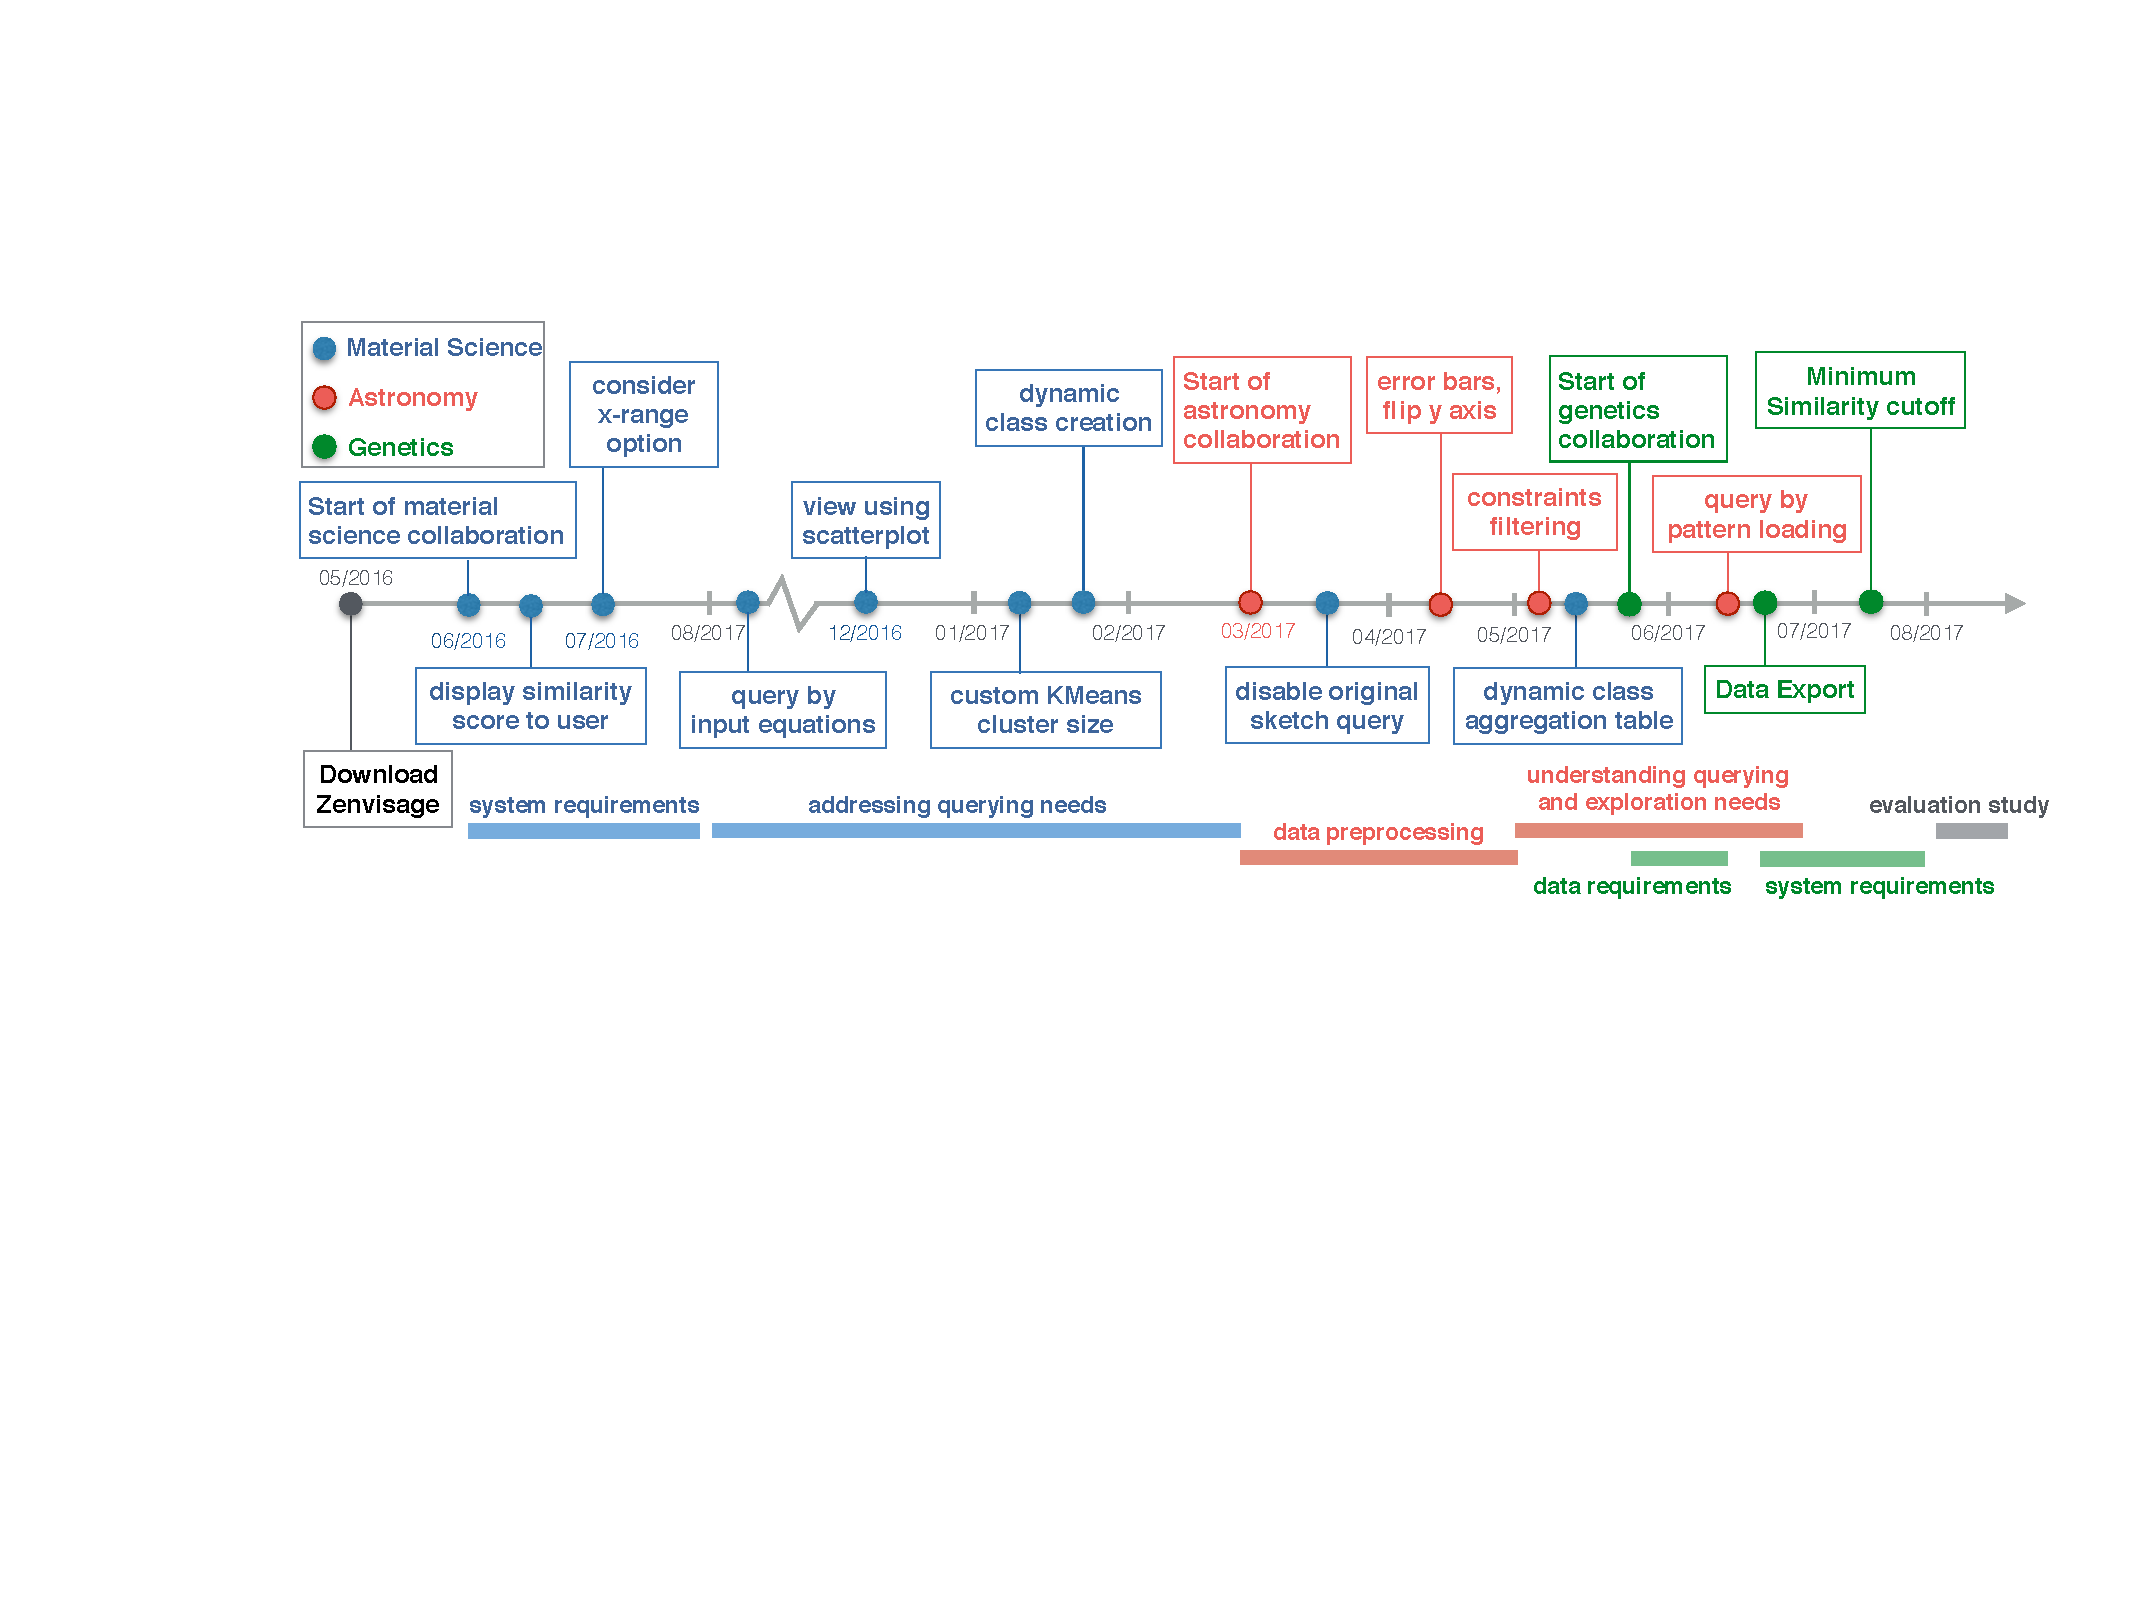
\includegraphics[width=6in]{figures/timeline_anon.pdf}
	\vspace{-6pt}\caption{Timeline for progress in participatory design studies.}
	\label{timeline}
	\vspace{-10pt}
\end{figure*}
\par Via cognitive walkthroughs and interviews, we first identified challenges in existing data analysis workflows in these domains
that could be potentially addressed by a VQS. Building on top of an existing, open-source VQS, \zv~\cite{Siddiqui2017,Siddiqui2017VLDB}, we collaborated closely with our participants to gather feedback and iterate on VQS feature designs,
over the course of a year, culminating in a new enhanced VQS, \zvpp. We organized these features into a taxonomy of VQS functionalities, involving three sensemaking processes inspired by Pirolli and Card's notional model of analyst sensemaking~\cite{Pirolli}. The sensemaking processes include top-down pattern specification (translating a pattern ``in-the-head'' into the form of a visual query), bottom-up data-driven inquiries (querying or recommending based on data), and context-creation (navigating across different collections of visualizations). We find that prior VQSs have focused largely on top-down processes, while largely ignoring the other two processes that are crucial for the needs in all three domains.
\par To study how various VQS features
are used in practice,
we conducted a final evaluation study with nine participants
using our final VQS prototype, \zvpp,
to address their research questions
on their own datasets.
In a 1.5-hour user study, participants were able to
gain novel scientific insights,
such as identifying a star with a transient pattern
that was known to harbor a Jupiter-sized planet
and finding characteristic gene expression profiles confirming the results of a related publication.\techreport{, and discovering that the dip in an astronomical light curve is caused by saturated imaging equipment overlooked by the existing error-detection pipeline.} \techreport{Participants also gain additional insights about their datasets, including debugging mislabeled features and uncovering erroneous data preprocessing procedure applied to a collaborator's dataset.}
%that goes from a pattern in-the-head to a desired visualization

\par By analyzing the evaluation study results, we discovered that sketching a pattern for querying is often ineffective. This is due to the fact that sketching makes the problematic assumptions that users know the pattern that they want to sketch and are able to sketch it precisely. Instead, participants typically opted for other means of pattern specification---one common mechanism was to drag-and-drop a recommended pattern onto the canvas, and then modify it (e.g., by smoothing it out). However, most VQSs do not support these other mechanisms (as we argued earlier, they typically focus only on top-down sensemaking processes, without covering bottom-up and context creation), partially explaining why such systems have not been widely adopted in practice.
\par Further analysis of how participants
transition between different sensemaking processes
during analysis---including the construction of a Markov Model---illustrated
how participants adopt a diverse set of workflows tailored
to their domains. We find that participants often construct analysis workflows focused around a primary sensemaking process, while iteratively interleaving their analysis with the two other processes. This finding points to how all three sensemaking processes, along with seamless transitions between them, are essential for enabling users to effectively use VQSs for data exploration.%For example, participants often center on a main sensemaking process, while interleaving variations with other two processes as they iterate on an analytic task.
\par To the best of our knowledge, our study is the \emph{first to holistically examine how VQSs can be designed to fit the needs of real-world
analysts and how they are actually used in practice}. Our contributions include:
\begin{denselist}
\item a characterization of the problems addressable by VQSs through design studies with three different domains,
\item the construction of a taxonomy of functionalities within VQSs, as well as an articulation of the problem space that is amenable to VQSs, both grounded in participatory design findings,
\item \change{an integrative} VQS, \zvpp, capable of facilitating rapid hypothesis generation and insight discovery,
\item study findings on how VQSs are used in practice, leading to the development of a novel sensemaking model for VQSs. %including the ineffectiveness of
%evaluation
% sketching and the ---- workflow
\end{denselist}
Our work not only opens up a new space of opportunities beyond the narrow use cases considered by prior studies, but also advocates common design guidelines and end-user considerations for building next-generation VQSs.
 %From these experiences, we  advocate visualization researchers and tool designers to ---- future VQS opportunities  Understanding the design space and opportunities for VQS
% Our three main research questions are as follows:

%and not as commonly ---- due to the --- challenges ----. that ----- characteristic workflows ---- iterative sensemaking loop.
%Our collaborative design experience culminated in a full-fledged VQS, \zvpp, described in Section~\ref{sec:pd_findings}.
% \noindent \emph{RQ1: What are the challenges in existing scientific data analysis workflows that could be potentially addressed by a VQS?}
% \par Via cognitive walkthroughs and interviews,
% we gained an understanding of the data analysis
% workflows presently employed by the scientists, their needs,
% and the challenges they face.
% We identified opportunities where a VQS could
% help accelerate their analysis, by helping them
% discover insights, gain intuition, or provoke directions
% for exploration. Finally, we determined the types of
% research questions and dataset properties that would
% be most suitable for exploration on VQSs.
%By learning about the needs and challenges that scientists face when working with their datasets through interviews and cognitive walkthroughs, we learned about the types of queries that they would like to pose on VQSs and distilled a set of design specifications that can better enable VQSs to help them discover insights, gain intuition about their datasets or provoke further directions for exploration. We also identify the types of research questions and dataset properties would be suitable for data exploration on VQSs.
% \begin{figure*}[ht!]
% \centering
% \vspace{-15pt}
% 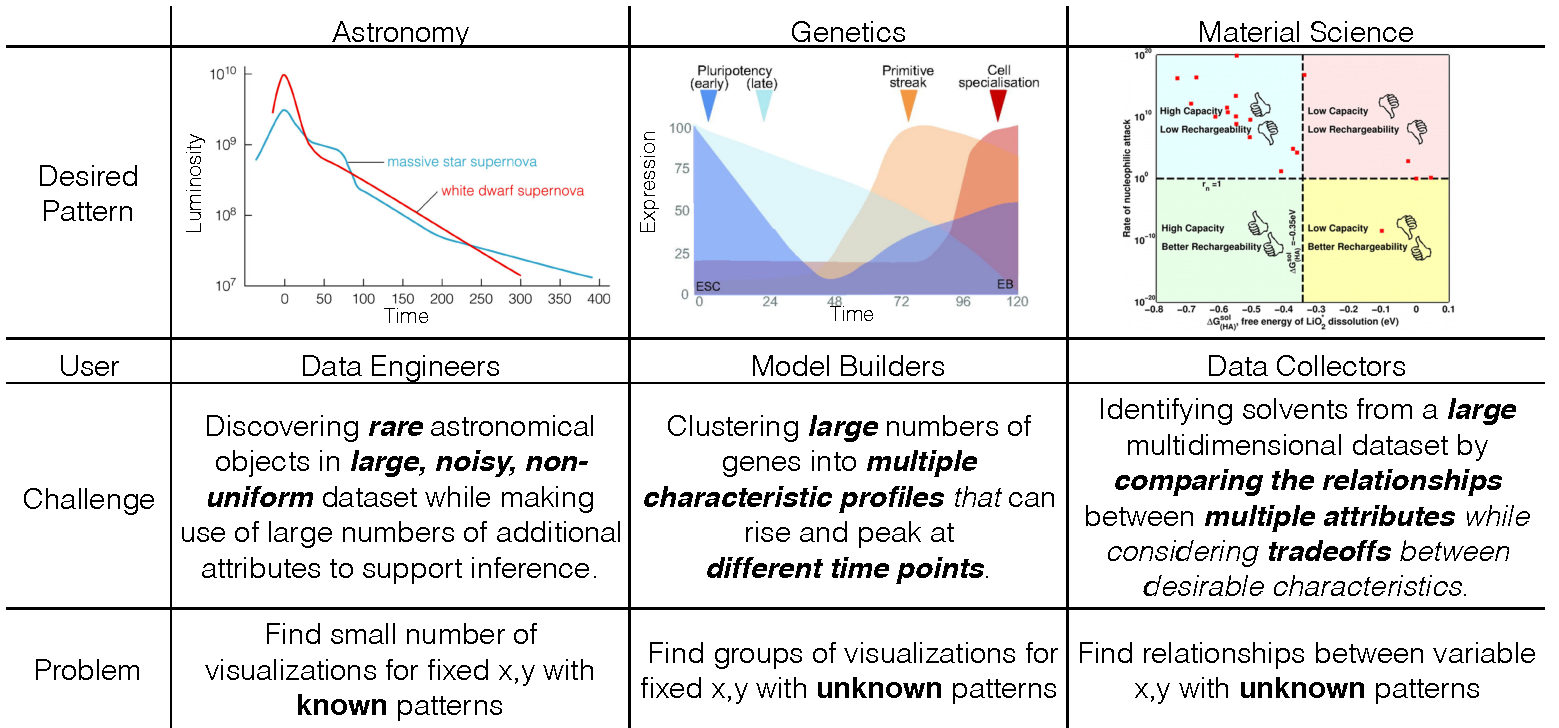
\includegraphics[width=0.8\linewidth]{figures/sci_challenge_tbl.pdf}
% \vspace{-6pt}\caption{Descriptions of the three scientific use cases discussed in this paper.}
% \label{example}
% \vspace{-10pt}
% \end{figure*}

% \noindent \emph{RQ2: What types of interface capabilities are necessary to develop VQSs into a useful component of data analysis?}
% \par Via participatory design, we distilled
% \tvcg{Based on our early interactions with scientists,
% we started to build a VQS~\cite{Siddiqui2017VLDB,Siddiqui2017} that, similar to existing VQSs~\cite{wattenberg2001sketching}, allowed them to search for desired trends via drawing on a canvas. This early system served as a functional prototype for us to engage with scientists further in the participatory design process, understand how they envision themselves using a VQS, and gather feedback on feature designs that could make the VQS more useful. The features we developed address challenges shared across the three scientific domains, ranging from additional querying modalities, to features that support a more integrated workflow, to improving the interpretability of the system output, \tvcg{most of them missing in} prior VQSs in the literature. Our collaborative design experience culminated in a full-fledged VQS, \zv, capable of facilitating rapid hypothesis generation and insight discovery.}

% \noindent \emph{RQ3: How do VQSs accelerate scientific insights?} and \emph{RQ4: How can VQSs fit within the context of existing data analysis workflows?}
% \\ To evaluate our final system \zv, we conducted a user study with nine scientists (including those who had participated in the design process), all of whom had a vested interest in using a VQS to address their research questions on their datasets. In a 1.5-hour user study, our scientist participants were able to gain novel scientific insights, such as \emph{\tvcg{identifying a star with a transient pattern that was known to harbor a Jupiter-sized planet,} finding characteristic gene expression profiles that confirmed the results of a related publication, and learning that the dip in an astronomical light curve is caused by saturated imaging equipment overlooked by the existing error-detection pipeline}.  Participants also gained additional insights about their datasets, including debugging \tvcg{mislabelled features and uncovering the erroneous data preprocessing procedure applied to a collaborator's dataset.}
% that the way data is aggregated across multiple experiments is erroneous on a collaborator's dataset.
% We learned how VQSs could be contextualized within scientific data analysis workflows and discovered that VQSs can be used beyond the exploratory phase of analysis, for data verification, debugging preliminary datasets, and performing sanity-checks on downstream models.

% \begin{figure}[h!]
%     \centering
%     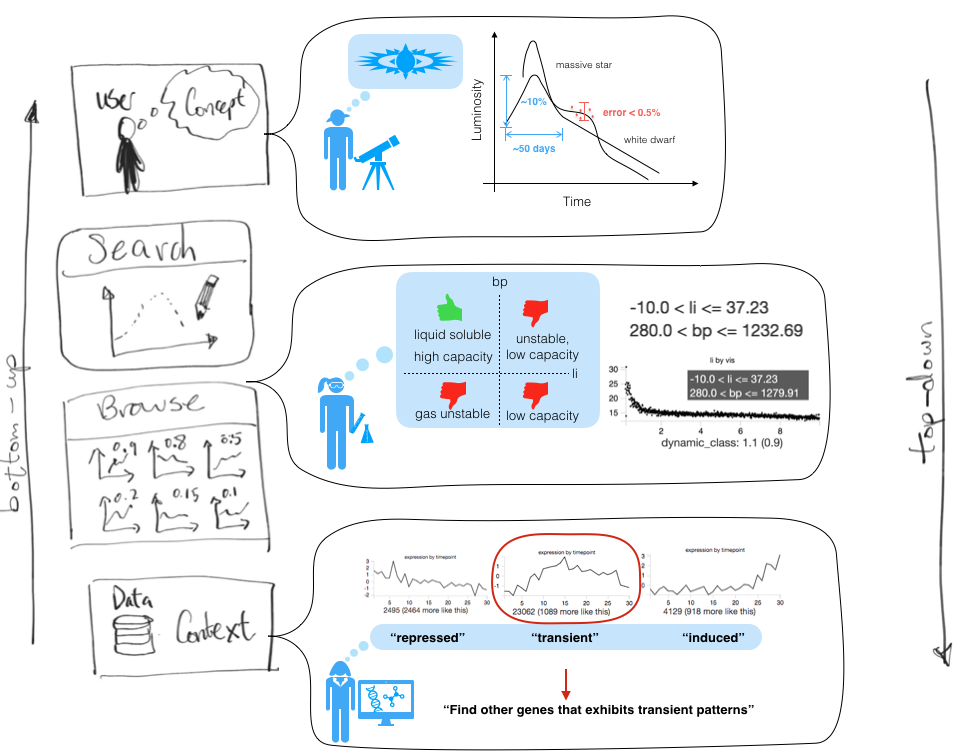
\includegraphics[width=\linewidth]{figures/search-browse-model.png}
%     \vspace{-6pt}\caption{Search Browse Model}
%     \label{fig:sbmodel}
%     \vspace{-5pt}
% \end{figure}

%!TEX root = main.tex
  \section{\change{Related Works\label{sec:relatedworks}}}
  % \subsection{Background and Motivation}
  \par \change{We will now describe past work in visual query systems and existing evaluation methods of visualization systems to provide background and motivation to our work.
  % Visual query systems enable users to directly search for visualizations matching certain patterns through an intuitive specification interface. Early work in this space focused on interfaces to search for time series with specific patterns.
  \par \emph{Visual query systems} (VQSs) is a term coined by Ryall et al. and Correll and Gleicher\cite{ryall2005querylines,correll2016semantics} to describe systems that enable analysts to directly search for time-series visualizations matching certain patterns through an intuitive specification interface. Examples of such systems} include TimeSearcher~\cite{Hochheiser2001,Hochheiser2004}, where the query specification mechanism is a rectangular box, with the tool filtering out all of the time series that does not pass through it, QuerySketch~\cite{wattenberg2001sketching} and Google Correlate~\cite{mohebbi2011google}, where the query is sketched as a pattern on canvas, with the tool filtering out all of the time series that have a different shape. Subsequent work recognized the ambiguity in sketching by studying how humans rank the similarity in patterns~\cite{Eichmann2015,correll2016semantics,Mannino2018} and improving the expressiveness of sketched queries through finer-grained specification interfaces and pattern-matching algorithms~\cite{ryall2005querylines,Holz2009}.
  %performed crowdsourced perceptual studies to understand how humans rank similarity in patterns subjectively
  % , including the use of soft constraints~\cite{ryall2005querylines} and implicit relaxed selection techniques~\cite{Holz2009}.
  % In addition to this ongoing work, recent work have also performed crowdsourced perceptual studies to understand how humans rank similarity in patterns subjectively~\cite{Eichmann2015,correll2016semantics,Mannino2018}.
  \par While these systems have been effective in controlled lab studies, they have never been designed and evaluated in-situ on multiple real-world use cases. Even when use cases were involved~\cite{Hochheiser2004,correll2016semantics}, the inclusion of these \change{case studies served as a post-hoc demonstrative case study that had} little influence on the major design decisions of the system. In the context of Munzner's nested model~\cite{munzner2009nested}, this \change{gap between research and adoption stems from} the common ``downstream threat'' of jumping prematurely into the deep levels of \textit{encoding, interaction, or algorithm design}, before a proper \textit{domain problem characterization} and \textit{data/operation abstraction design} is performed. In this work, we performed design studies~\cite{lam2012empirical,shneiderman2006strategies,Sedlmair2012} with three different subject areas for \textit{domain problem characterization}. Comparing and contrasting between the diverse set of questions, datasets, and challenges across these three use cases revealed new generalizable insights and enabled us to better understand how VQSs can be extended for novel and unforeseen use cases. Based on these findings, we developed a taxonomy for understanding the sensemaking process in VQSs as part of the \textit{data/operation abstraction design}. Finally, we validated the abstraction design with grounded evaluation~\cite{Plaisant2004,Isenberg2008}, where we invited participants to bring in their own datasets and research problems that they have a vested interest in to test our final deployed system. \change{Next, we will outline these two phases of our study, deferring details of the study procedures and protocols to the technical report.}%Next, we will describe these two phases of our study in more detail.
  %had a narrow objective and had 
  \begin{table}[h!]
    \vspace*{-10pt}
     \centering
     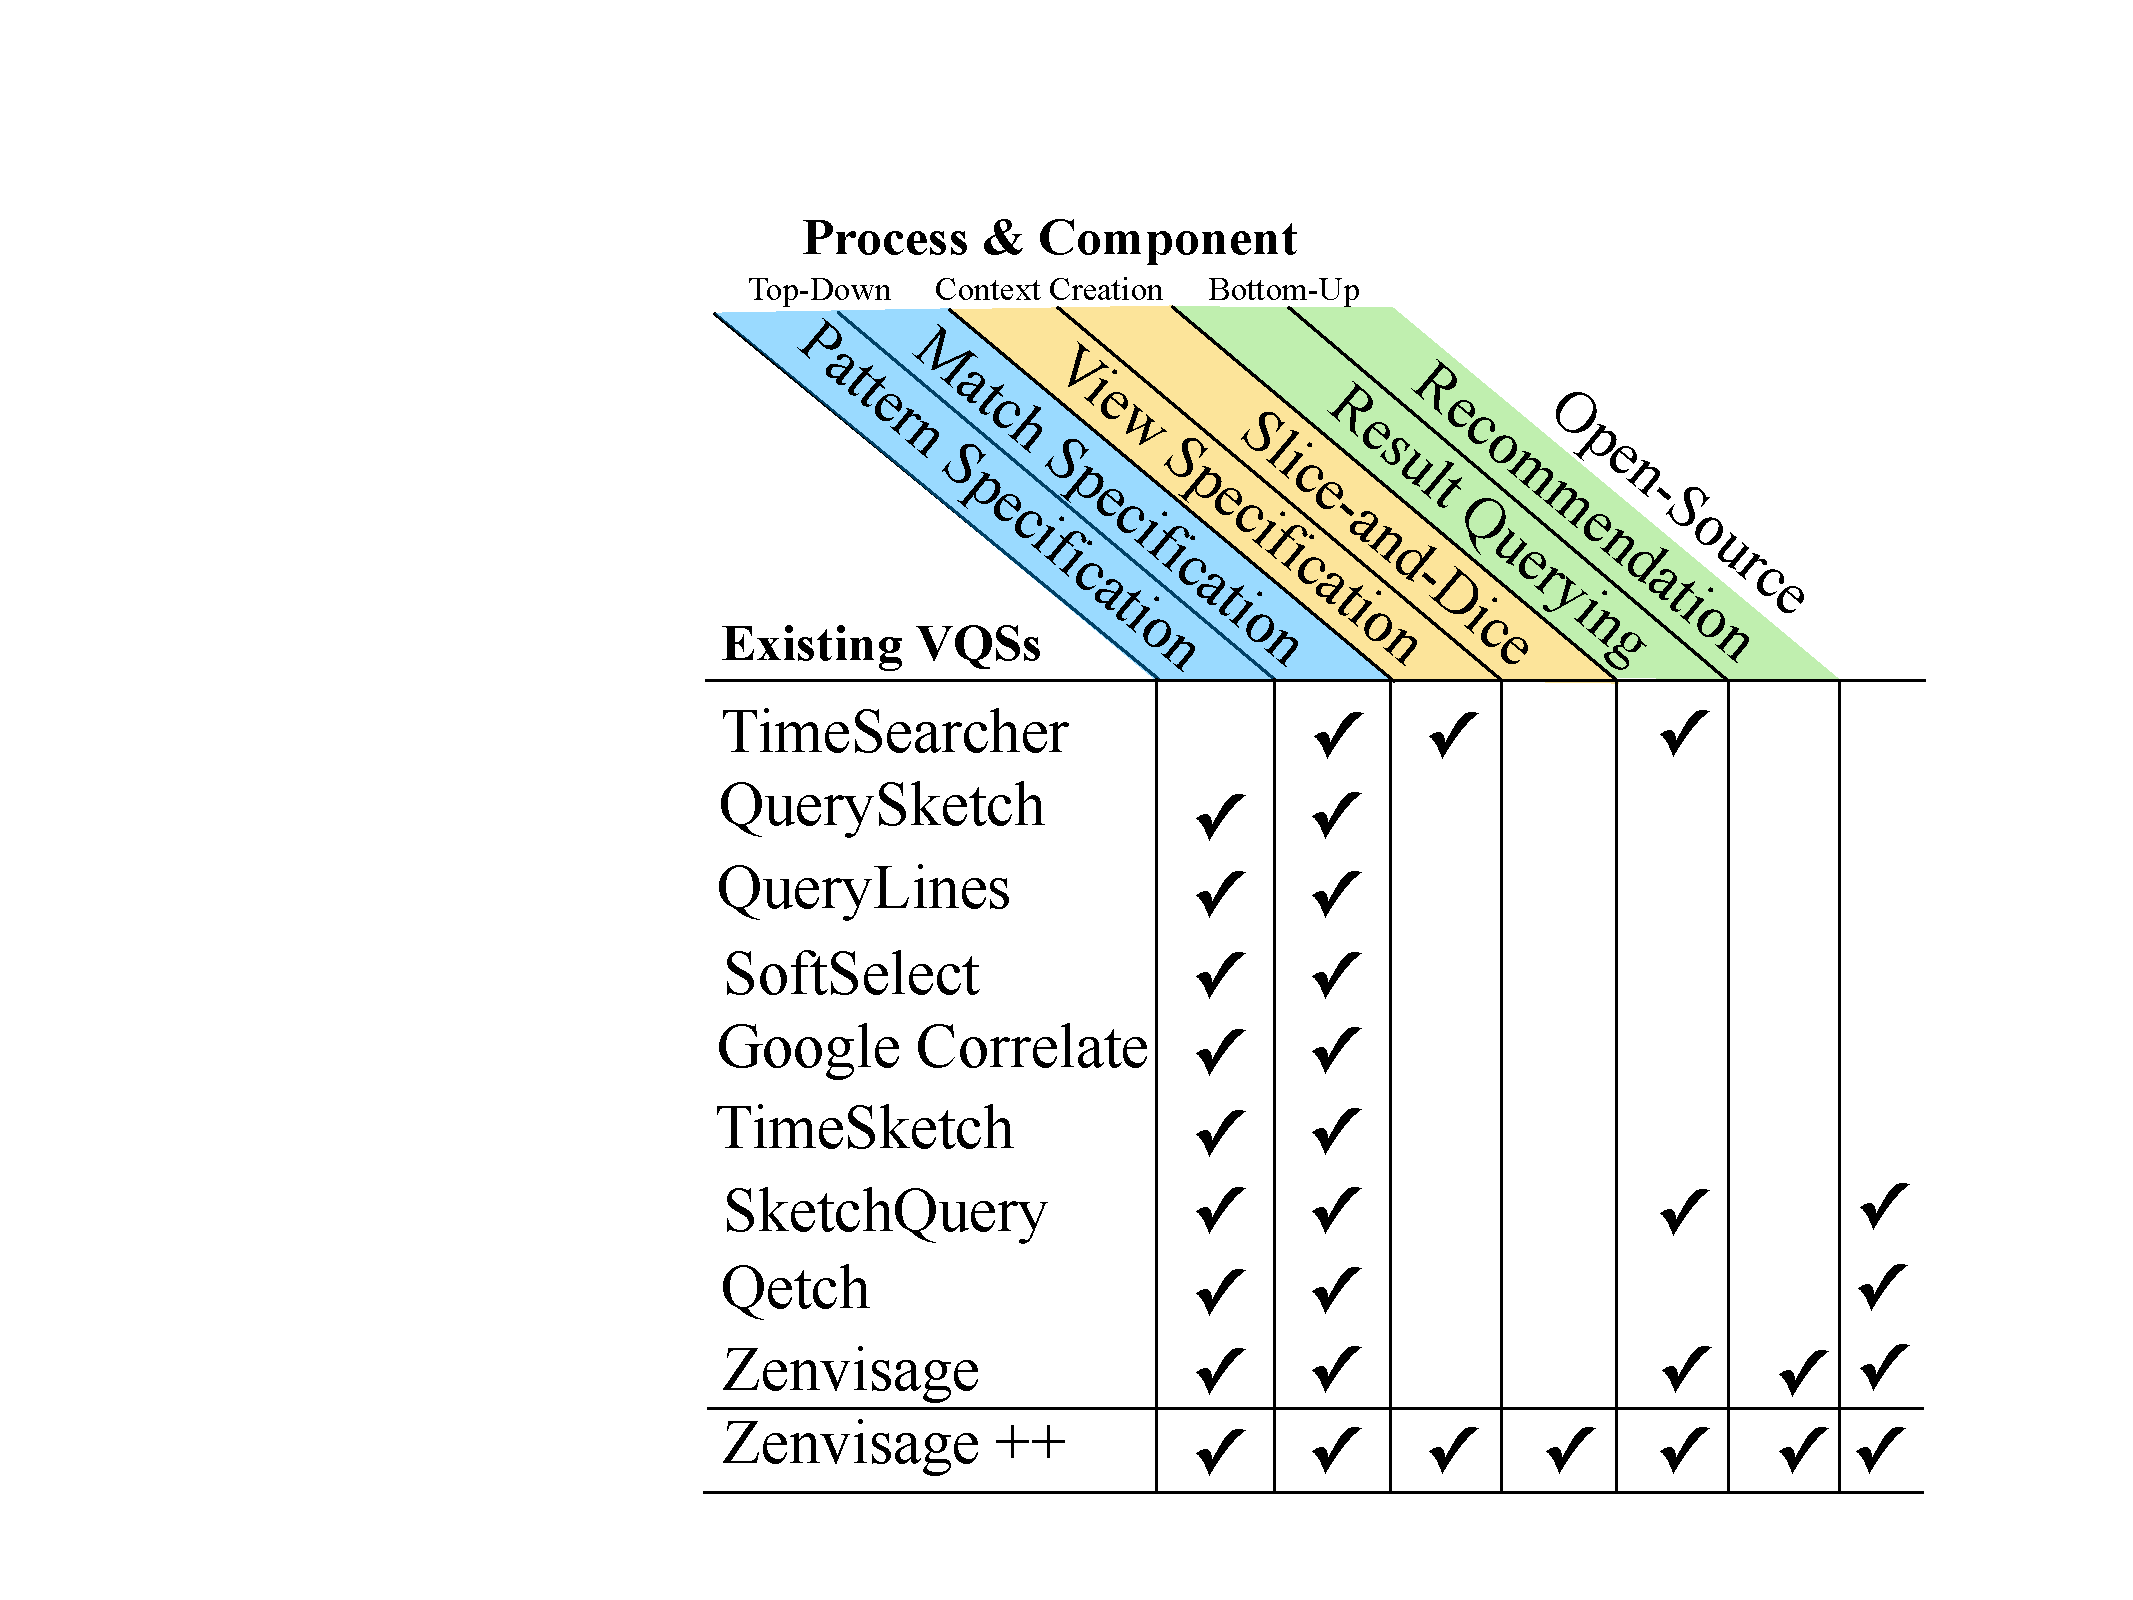
\includegraphics[width=0.8\linewidth]{figures/related_works_table.pdf}
     \caption{Table summarizing whether key functional components (columns) are covered by past systems (row), indicated by checked cells. Column header colors blue, orange, green represents three sensemaking process (top-down querying, search with context, and bottom-up querying) described in Section~\ref{sec:pd_findings}. The heavily-used, practical features in our study for context-creation and bottom-up inquiry is largely missing from prior VQSs.}
     \label{table:relatedwork}
     \vspace*{-15pt}
 \end{table}
%!TEX root = main.tex
\tvcg{\section{Methods} \label{methods}}
%\subsection{Evaluation Methods For Visualization Systems}
\tvcg{\subsection{Methodology Background\label{methodology_relatedwork}}}
\par Visualization systems are often evaluated using controlled studies that measure the user's performance against an existing visualization baseline~\cite{Plaisant2004}. Cognitive measures such as insight time~\cite{North2006,Yi2008} have been developed to capture how well users perform on a task against existing baselines. However, since the operations, hypotheses generated, and insights obtained through exploratory analysis are variable and subjective to individual users and their analytic goals, it is impossible to define tasks beforehand and compare across control groups. Techniques such as artificially inserting ``insights'' or setting predefined tasks for example datasets work well for objective tasks, such as debugging data errors~\cite{kandel2011wrangler,Patel2010}, but this contrived method is unsuitable for trying to learn about the types of real-world queries a user may want to pose on a VQS. \techreport{In order to make the user study more realistic, we opted for a qualitative evaluation where we allowed participants to bring a dataset that they have a vested interest in to address an unanswered research question.}
\par Due to the unrealistic nature of controlled studies, many have proposed using a more multi-faceted, ethnographic approach to understand how analysts perform visual data analysis and reasoning~\cite{Plaisant2004,lam2012empirical,shneiderman2006strategies,munzner2009nested,Sedlmair2012}. For example, multi-dimensional, in-depth, long-term case studies (MILCs) advocate the use of interviews, surveys, logging and other empirical artifacts to create a holistic understanding of how a visualization system is used in its intended environment \cite{shneiderman2006strategies}. Some papers have explored designing visualization and collaborative tools for scientific workflows through individual case studies, e.g.,~\cite{Poon2008,Chen2016}. Similarly, in our work, real-world case studies help us situate how VQSs could be used in the context of an existing analysis workflow.  
\par We adopt {\em participatory design} practices in this work: participatory design ``allows potential users to 
 participate in the design of a system that they will ultimately use''~\cite{Gould1983,Muller1993}. Participatory design has been successfully used in the development of interactive visualization systems in the past~\cite{Aragon2008,Chuang2012}. \tvcg{\cite{Sedlmair2012} highlights the benefits and pitfalls of design study. They advocate that design study methodology is suitable for use cases in which the data is available for prototyping, but the task is only partially known and information is partially in the user's head. In that regard, our scientific use cases with VQS is well-suited for a design research methodology, as we learn about the scientist's data and analysis requirements and design interactions that helps users elicit their ``in-the-head'' specifications into actionable visual queries.} %\cut{In this work, we collaborated with scientists early on to develop features in \zv that address their analysis needs.}  
\tvcg{\subsection{Our Approach}}
\par We adopted a mixed methods research methodology that draws inspiration from ethnographic methods, iterative and participatory design, and controlled studies~\cite{jorgensen_2008,miller_salkind_miller_2002,shneiderman2006strategies,Muller1993} to understand how VQSs can accelerate scientific data analysis. Our methodology served to address the research questions outlined in the introduction. Working with researchers from three different scientific research groups, we identified the needs and challenges of scientific data analysis and the potential opportunities for VQSs to fit in, via interviews and cognitive walkthroughs{\em (RQ1)}. We further extended an existing VQS, \zv, with features for scientists via participatory design{\em (RQ2)}  
\par \tvcg{We chose to build on top of \zv as functional prototype in the design study. The use of functional prototypes is common in participatory design to provide a starting point for the participants. For example, \cite{Ciolfi2016} studied two different alternatives to co-design (starting with open brief versus functional prototype) in the development of museum guidance systems and found that while both approaches were equally fruitful, functional prototypes can make addressing a specific challenge more immediate and focused (in our case the challenge is making comparison across large numbers of visualizations as we found in through informal discussions with practitioners). Our motivation for providing a functional prototype at the beginning of the participatory design sessions is to showcase capabilities of VQSs. Especially since VQSs are not uncommon in the existing workflow of these scientists, participants may not be able to imagine their use cases without a starting point.} %\sout{our prototypical VQS, since it is open-source, has both canvas-based querying capabilities as well as visualization recommendations. (\zv also has a sophisticated query language, ZQL, that we did not employ.)} 
\par As shown in Figure \ref{oldZV}, the basic version of \zv that we built on allowed users to sketch a pattern or drag-and-drop an existing visualization as a query, and \zv would then return visualizations that had the closest Euclidean distance from the queried pattern. The system also displayed representative and outlier patterns to help provide  an overview of typical trends.
	\begin{figure}[ht!]
	\centering
	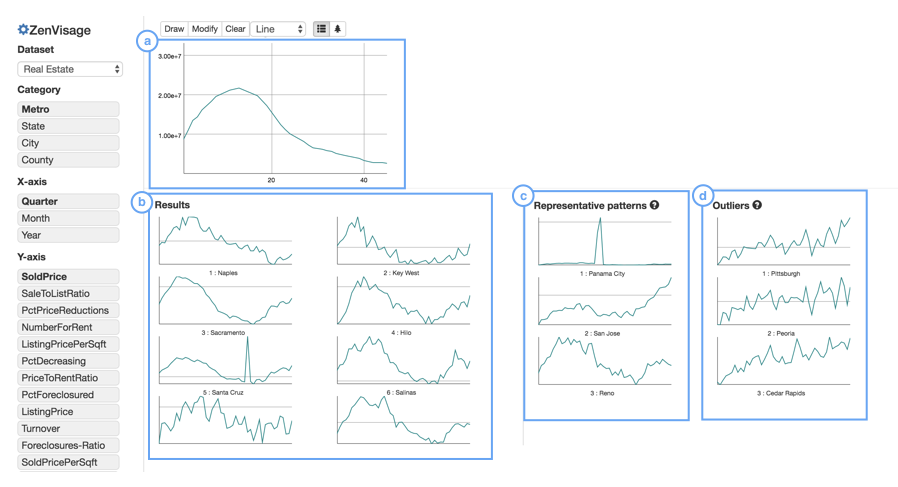
\includegraphics[width=\linewidth]{figures/oldZV_nozql.png}
	\caption{The basic version of \zv that we built on top of allowed users to sketch a pattern in (a), which would then return (b) results that had the closest Euclidean distance from the sketched pattern. The system also displays (c) representative patterns obtained through K-means clustering and (d) outlier patterns to help the users gain an overview of the dataset. \tvcg{The details of the system is described in our previous work \cite{Siddiqui2017,Siddiqui2017VLDB}.}}
	\label{oldZV}
	\end{figure}
\par After incorporating desired features into \ourVQS over the period of a year, we conducted a qualitative evaluation to study how our improved VQS affected the way the users explore their data{\em (RQ3,4)} . \cut{It is interesting to note that not all of the features suggested by the participants were found to be useful during our evaluation.}
\begin{table}[h]
\centering
\vspace{-10pt}
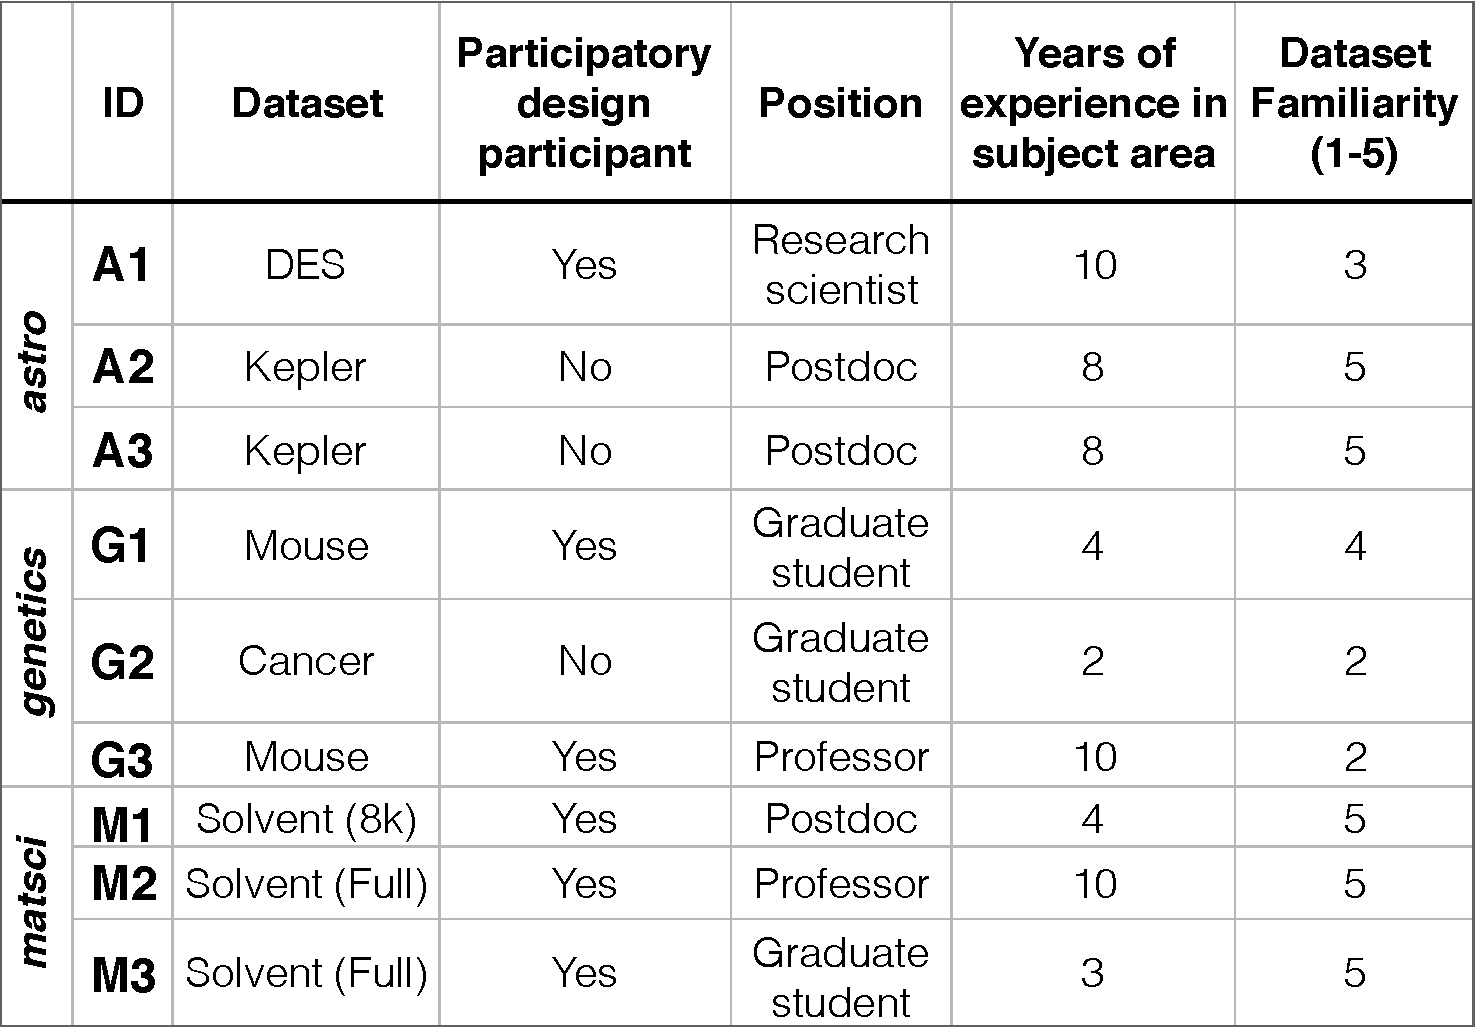
\includegraphics[width=\linewidth]{figures/participants.pdf}
\caption{Participant information. The Likert scale used for dataset familiarity ranges from 1 (not at all familiar) to 5 (extremely familiar).}
\label{participants}
\vspace{-10pt}
\end{table}
\tvcg{\section{Understanding Scientific Data Analysis (R1)}}
%\cut{ \subsection{Understanding Scientific Data Analysis}
%\par Our initial inspiration for building a VQS came from informal discussions with many academic and industry analysts. Their current workflows required the analysts to manually examine a large number of visualizations to derive insights from their data. In this section, we address RQ1 by understanding the limitations and opportunities in existing scientific data analysis workflows in three research areas. We begin by describing the participants in these areas.} 
\subsection{Participants, Datasets and Workflows}
We recruited participants by reaching out to research groups who were interested in using VQSs for exploring their data via email.\dor{Not sure if we should make this more general about challenges in data analysis rather than focus on VQS to correspond to our earlier statement.} We summarize the common properties and differences of these three groups of researchers in Figure~\ref{example} and the desirable characteristics common to these datasets suitable for VQSs in \tvcg{the Section~\ref{metastudy}}. Six scientists from three research groups participated in the design of \zv. The evaluation study participants included these six scientists, along with three ``blank-slate'' participants who had never encountered \zv before. While participatory design subjects actively provided feedback on \zv with their data, they only saw us demonstrating their requested features and explaining the system to them, rather than actively using the system on their own. So the evaluation study was the first time that all nine of the participants used \zv to explore their datasets. We list the participants in Table~\ref{participants}, and refer to them by their anonymized ID as listed in the table. 
\techreport{On average, the participants had more than 8 years of experience working in their respective fields.}
\begin{figure*}[ht!]
\centering
\vspace{-10pt}
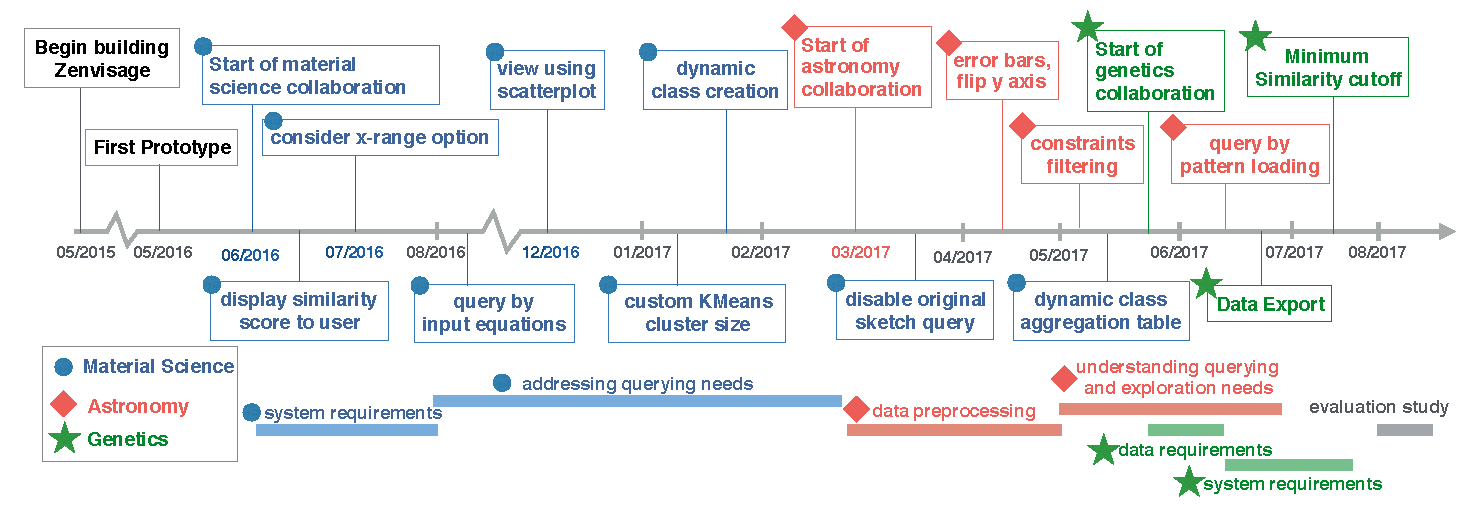
\includegraphics[width=6in]{figures/timeline_new.pdf}
\vspace{-6pt}\caption{Participatory design timeline for the scientific use cases.}
\label{timeline}
\vspace{-10pt}
\end{figure*}

\techreport{The research questions and objectives of the participants were diverse even among those in the same subject area and using the same dataset. Examples of research questions included: 
\begin{denselist}
\item Understanding the gene expression profiles of breast cancer cells that exhibit induced, transient, and  repressed patterns after a particular treatment.
\item Studying common patterns among stars that exhibit planetary transits versus stars that don't from the Kepler space telescope\footnote{\url{www.nasa.gov/mission_pages/kepler/main/index.html}}.
\item Identifying battery solvents with favorable properties and mass production potential through studying how changes in certain chemical properties correlate to changes in other chemical properties. \end{denselist}
}
\par The pre-study survey with the participants showed that out of all of the steps in their data analysis workflow\footnote{This includes viewing and browsing data, data cleaning and wrangling, computing statistics, data visualization, and model building or machine learning.}, they spend the most time computing statistics and creating visualizations.
The main bottlenecks cited in their existing workflow included the challenge of dealing with large amounts of data, writing custom processing and analysis scripts, and long turnaround times incurred by making modifications to an upstream operation in a segmented workflow. \ccut{On average, participants expressed interest in adopting \zv in their day-to-day workflow as eight from a Likert scale of ten after the study \kk{not sure what this means}.}
\par During the participatory design process, we collaborated with each of the teams closely with an average of two meetings per month, where we learned about their datasets, objectives, and how VQSs could help address their research questions. A detailed timeline of our engagement with the participants and the features inspired by their use cases can be found in Figure \ref{timeline}. Participants provided datasets they were exploring from their domain, whereby they had a vested interest to use a VQS to address their own research questions. We  describe the three scientific use cases below.

\par \textbf{Astronomy (\astro):} The Dark Energy Survey (DES) is a multi-institutional project with over 400 scientists. Scientists use a multi-band telescope that takes images of 300 million galaxies over 525 nights to study dark energy\cite{Drlica-Wagner2017}. The telescope also focuses on smaller patches of the sky on a weekly interval to discover astrophysical transients (objects whose brightness changes dramatically as a function of time), such as supernova explosions or quasars. The output is a time series of brightness observations associated with each object extracted from the images observed. %\kk{is it 4 years of 525 nights?}\dor{it's a bit confusing, because they only observe half a year on the southern hemisphere, will skip talking about this} 

For over five months, we worked closely with an astronomer on the project's data management team working at a supercomputing facility. \cut{We also gathered feedback from other astronomers who were interested in studying the properties of astrophysical transients during a collaboration-wide meeting.} The scientific goal is to identify a smaller set of potential candidates that may be astrophysical transients in order to study their properties in more detail. These insights can help further constrain physical models regarding the formation of these objects.
\par \textbf{Genetics (\bio):} Gene expression is a common data type used in genomics and is obtained via microarray experiments. \techreport{In these experiments, a grid containing thousands of DNA fragments are exposed to stimuli and measurements for the level at which a gene is expressed are recorded as a function of time.} The data used in the participatory design sessions was the gene expression data over time for mouse stem cells aggregated over multiple experiments, downloaded from an online database\footnote{\url{ncbi.nlm.nih.gov/geo/}}. 
\par  We worked with \tvcg{a graduate student and a PI} at a research university over three months who were using gene expression data to better understand how genes are related to phenotypes expressed during early development~\cite{Peng2016,Gloss084442}. They were interested in using \zv to cluster gene expression data before conducting analysis with a downstream machine learning workflow. 
\par \textbf{Material Science (\matsci):} We collaborated with material scientists at a research university who are working to identify solvents that can improve battery performance and stability. These scientists work with large datasets containing over 25 chemical properties for more than 280K different solvents obtained from simulations. \techreport{Once they have identified a solvent that also produces favorable results in an experiment, they identify other solvents with similar properties,  which may be cheaper or safer to manufacture at an industrial scale.}
\par We worked closely with two graduate students and a PI for over a year to design a sensible way of exploring their data using VQSs\footnote{Note that while we have interacted with the \matsci participant during the initial development stage, the participatory design formally started in June 2016}. Each row of their dataset represents a unique solvent, and consists of 25 different chemical attributes. They wanted to use \zv to identify solvents which have similar properties to known solvents but are more favorable (e.g. cheaper or safer to manufacture), and identify how changes in certain chemical attributes affects them.
\raggedbottom

%%%%%%%%%%%%%%%%%%%%%%%%%%%%%%%%%
\subsection{Cognitive Walkthrough Sessions}
Cognitive walkthroughs highlight the existing workflows and behavior that participants have adopted for conducting certain tasks~\cite{Nielsen1994}. In our case, we observed the participants as they conducted a cognitive walkthrough demonstrating every component of their current data analysis workflow.
\techreport{
	\begin{figure}[ht!]
		\centering
		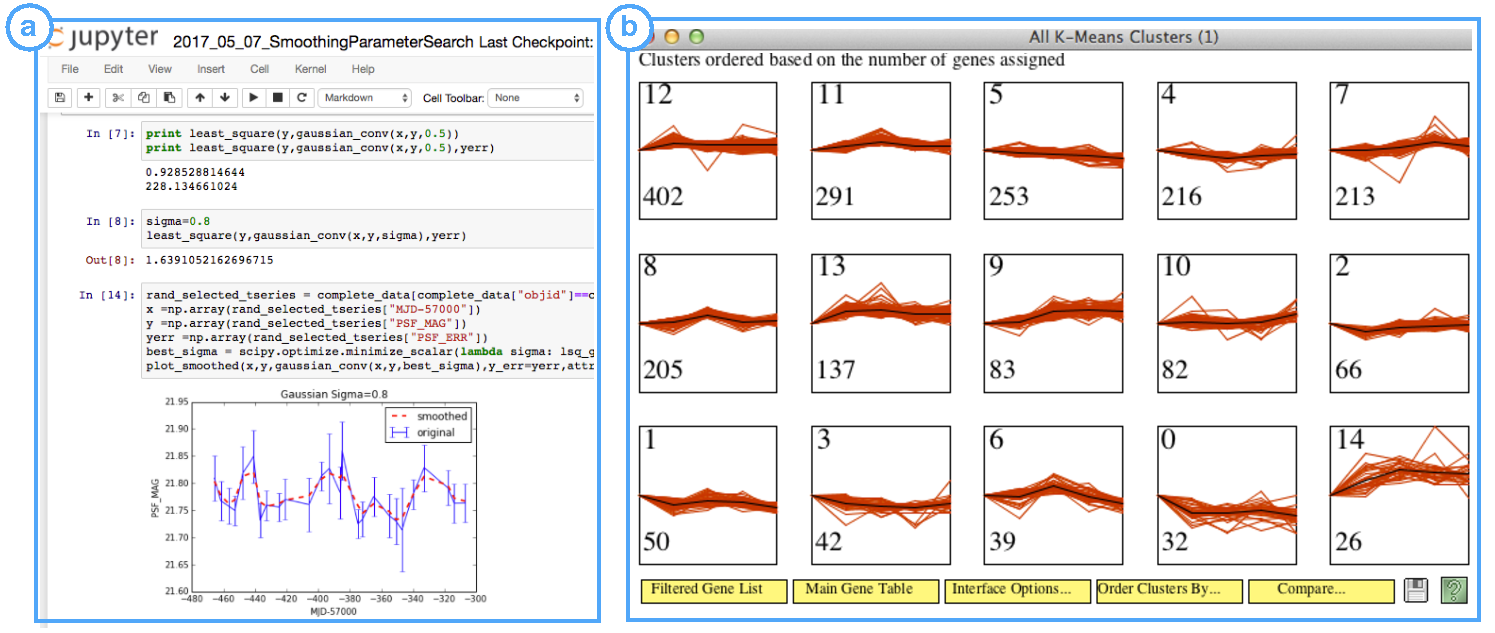
\includegraphics[width=\linewidth]{figures/workflow.pdf}
		\caption{Examples of the scientists' original workflow: a) The astronomer performs various data analysis task using the Jupyter notebook environment, b) The geneticists uses a domain-specific software to examine clustering outputs.}
		\label{workflow}
	\end{figure}
}
\par \textbf{Astronomy:} Since astronomical datasets are often terabytes in scale, they are often processed and stored in highly specialized data management centers in supercomputing centers. The collaboration's data management team has created a command-line interface that enables users to easily query, browse, and download their data\techreport{\footnote{ \url{github.com/mgckind/easyaccess}}}. 
After the data is downloaded, most of the work is done programmatically through Python in an interactive Jupyter notebook environment\footnote{\url{jupyter.org}}. The astronomer inspects the data schema, performs data cleaning and  wrangling, computes relevant statistics, and generates visualizations to search for anomalies or objects of interest, as shown in Figure \ref{workflow}a.
\par While an experienced astronomer who has examined many transient light curves can often distinguish an interesting transient object from noise by sight, they must visually examine and iterate through large numbers of visualizations of candidate objects. Manual searching is time-consuming and error prone as the majority of the objects will not be astronomical transients.
Participant A1 was interested in \zv as he recognized how specific pattern queries could help scientists directly search for these rare objects. 
\techreport{\par If an object of interest or region is identified through the visual analysis, then the astronomer may be interested in inspecting the image of the region for cross-checking that the significant change in brightness of the object is not due to an imaging artifact. This could be done using a custom built web-interface that facilitates the access of cutout images for a queried region of the sky.} 

\par \textbf{Genetics:} Participant G1 processes the raw microarray data by using a preprocessing script written in R \techreport{, where they (i) sub-select 144 genes of interest, (ii) clean up an experimental artifact due to measurements on multiple probes, (iii) log-transform the raw data to show a more distinct shape profile for clustering, (iv) normalize the gene expression values into the range of 0 to 1, and (v) perform Loess smoothing with default parameters to reduce the noise in the data}. To analyze the data, the preprocessed data is loaded into a desktop application for visualizing and clustering gene expression data\footnote{ \url{www.cs.cmu.edu/~jernst/stem/}}. G1 sets several clustering and visualization parameters on the interface before pressing a button to execute the clustering algorithm. The cluster visualizations are then displayed as overlaid time series for each cluster, as shown in the visualization in Figure \ref{workflow}b. G1 visually inspects that all the patterns in each cluster look ``clean'' and checks the number of outlier genes that do not fall into any of the clusters.  If the number of outliers is high or the visualizations look unclean, they rerun the clustering by increasing the number of clusters. Once the visualized clusters look ``good enough'', G1 exports the cluster patterns into a csv file to be used as features in their downstream regression tasks.
\par Prior to the study, the student (G1) and PI (G3) spent over a month attempting to determine the best number of clusters for their upstream analysis based on a series of static visualizations and statistics computed after clustering. While regenerating their results took no more than 15 minutes every time they made a change, the multi-step, segmented workflow meant that all changes had to be done offline, so that valuable meeting time was not wasted trying to regenerate results. The team had a vested interest in participating in the design of \zv as they saw how the interactive nature of VQSs and the ability to query other time series with clustering results could dramatically speed up their collaborative analysis process. 
\par \textbf{Material Science:} Participant M1 starts his data exploration process with a list of known and proven solvents as a reference. For instance, he would search for solvents which have boiling point over 300 Kelvins and the lithium solvation energy under 10 kcal/mol using basic SQL queries. This would help him narrow down the list of solvents, and he would continue this process with other properties. The scientist also considers the availability and the cost of the solvents while exploring the dataset. When the remaining list of the solvents is sufficiently small, he drills down to more detail (e.g., such as looking at the chemical structure of the solvents to consider the feasibility of conducting experiments with the solvent). While he had identified potential solvents through  manual lookup and comparison,  the process lacked the ability to reveal complicated trends and patterns that might be hidden, such as how the change in one attribute can affect the behavior of other attributes of a solvent. M1 was interested in using a VQS as it was infeasible for him to manually compare between large numbers of solvents and their associated properties manually.
\raggedbottom
%!TEX root = main.tex
\tvcg{\section{Understanding Scientific Data Analysis (R1)}}
%\cut{ \subsection{Understanding Scientific Data Analysis}
%\par Our initial inspiration for building a VQS came from informal discussions with many academic and industry analysts. Their current workflows required the analysts to manually examine a large number of visualizations to derive insights from their data. In this section, we address RQ1 by understanding the limitations and opportunities in existing scientific data analysis workflows in three research areas. We begin by describing the participants in these areas.} 
\subsection{Participants, Datasets and Workflows}
We recruited participants by reaching out to research groups who were interested in using VQSs for exploring their data via email. \kk{Need to be more explicit about recruitment strategy here?}\tvcg{As described in more detail in Section \ref{metastudy}, we initially spoke to analysts from 12 different potential application area and narrowed down to three use cases in astronomy, genetics, and material science for our participatory design study.} We summarize the common properties and differences of these three groups of researchers in Figure~\ref{example} and the desirable characteristics common to these datasets suitable for VQSs in \tvcg{the Section~\ref{metastudy}}. Six scientists from three research groups participated in the design of \zv. The evaluation study participants included these six scientists, along with three ``blank-slate'' participants who had never encountered \zv before. While participatory design subjects actively provided feedback on \zv with their data, they only saw us demonstrating their requested features and explaining the system to them, rather than actively using the system on their own. So the evaluation study was the first time that all nine of the participants used \zv to explore their datasets. We list the participants in Table~\ref{participants}, and refer to them by their anonymized ID as listed in the table. 
\techreport{On average, the participants had more than 8 years of experience working in their respective fields.}
\begin{figure*}[ht!]
\centering
\vspace{-10pt}
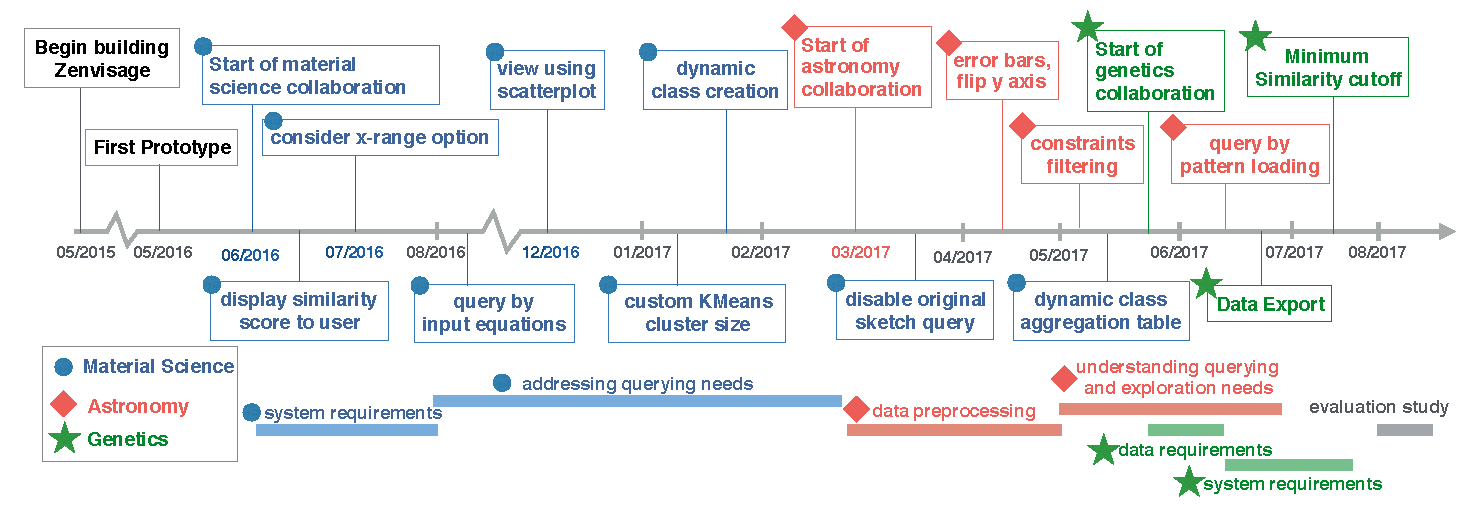
\includegraphics[width=6in]{figures/timeline_new.pdf}
\vspace{-6pt}\caption{Participatory design timeline for the scientific use cases.}
\label{timeline}
\vspace{-10pt}
\end{figure*}

\techreport{The research questions and objectives of the participants were diverse even among those in the same subject area and using the same dataset. Examples of research questions included: 
\begin{denselist}
\item Understanding the gene expression profiles of breast cancer cells that exhibit induced, transient, and  repressed patterns after a particular treatment.
\item Studying common patterns among stars that exhibit planetary transits versus stars that don't from the Kepler space telescope\footnote{\url{www.nasa.gov/mission_pages/kepler/main/index.html}}.
\item Identifying battery solvents with favorable properties and mass production potential through studying how changes in certain chemical properties correlate to changes in other chemical properties. \end{denselist}
}
\par The pre-study survey with the participants showed that out of all of the steps in their data analysis workflow\footnote{This includes viewing and browsing data, data cleaning and wrangling, computing statistics, data visualization, and model building or machine learning.}, they spend the most time computing statistics and creating visualizations.
The main bottlenecks cited in their existing workflow included the challenge of dealing with large amounts of data, writing custom processing and analysis scripts, and long turnaround times incurred by making modifications to an upstream operation in a segmented workflow. \ccut{On average, participants expressed interest in adopting \zv in their day-to-day workflow as eight from a Likert scale of ten after the study \kk{not sure what this means}.}
\par During the participatory design process, we collaborated with each of the teams closely with an average of two meetings per month, where we learned about their datasets, objectives, and how VQSs could help address their research questions. A detailed timeline of our engagement with the participants and the features inspired by their use cases can be found in Figure \ref{timeline}. Participants provided datasets they were exploring from their domain, whereby they had a vested interest to use a VQS to address their own research questions. We  describe the three scientific use cases below.

\par \textbf{Astronomy (\astro):} The Dark Energy Survey (DES) is a multi-institutional project with over 400 scientists. Scientists use a multi-band telescope that takes images of 300 million galaxies over 525 nights to study dark energy\cite{Drlica-Wagner2017}. The telescope also focuses on smaller patches of the sky on a weekly interval to discover astrophysical transients (objects whose brightness changes dramatically as a function of time), such as supernova explosions or quasars. The output is a time series of brightness observations associated with each object extracted from the images observed. %\kk{is it 4 years of 525 nights?}\dor{it's a bit confusing, because they only observe half a year on the southern hemisphere, will skip talking about this} 

For over five months, we worked closely with an astronomer on the project's data management team working at a supercomputing facility. \ccut{We also gathered feedback from other astronomers who were interested in studying the properties of astrophysical transients during a collaboration-wide meeting.} The scientific goal is to identify a smaller set of potential candidates that may be astrophysical transients in order to study their properties in more detail. These insights can help further constrain physical models regarding the formation of these objects.
\par \textbf{Genetics (\bio):} Gene expression is a common data type used in genomics and is obtained via microarray experiments. \techreport{In these experiments, a grid containing thousands of DNA fragments are exposed to stimuli and measurements for the level at which a gene is expressed are recorded as a function of time.} The data used in the participatory design sessions was the gene expression data over time for mouse stem cells aggregated over multiple experiments, downloaded from an online database\footnote{\url{ncbi.nlm.nih.gov/geo/}}. 
\par  We worked with \tvcg{a graduate student and a PI} at a research university over three months who were using gene expression data to better understand how genes are related to phenotypes expressed during early development~\cite{Peng2016,Gloss2017}. They were interested in using \zv to cluster gene expression data before conducting analysis with a downstream machine learning workflow. 
\par \textbf{Material Science (\matsci):} We collaborated with material scientists at a research university who are working to identify solvents that can improve battery performance and stability. These scientists work with large datasets containing over 25 chemical properties for more than 280k different solvents obtained from simulations. \techreport{Once they have identified a solvent that also produces favorable results in an experiment, they identify other solvents with similar properties,  which may be cheaper or safer to manufacture at an industrial scale.}
\par We worked closely with a graduate students, a postdoctoral researcher, and a PI for over a year to design a sensible way of exploring their data using VQSs\footnote{Note that while we have interacted with the \matsci participant during the initial development stage, the participatory design formally started in June 2016}. Each row of their dataset represents a unique solvent, and consists of 25 different chemical attributes. They wanted to use \zv to identify solvents which have similar properties to known solvents but are more favorable (e.g. cheaper or safer to manufacture), and identify how changes in certain chemical attributes affects them.
\raggedbottom

%%%%%%%%%%%%%%%%%%%%%%%%%%%%%%%%%
\subsection{Cognitive Walkthrough Sessions}
\tvcg{During the design study, we observed the participants as they conducted a cognitive walkthrough demonstrating every component of their current data analysis workflow. Cognitive walkthroughs highlight the existing workflows and behavior that participants have adopted for conducting certain tasks~\cite{Nielsen1994}.}
\techreport{
	\begin{figure}[ht!]
		\centering
		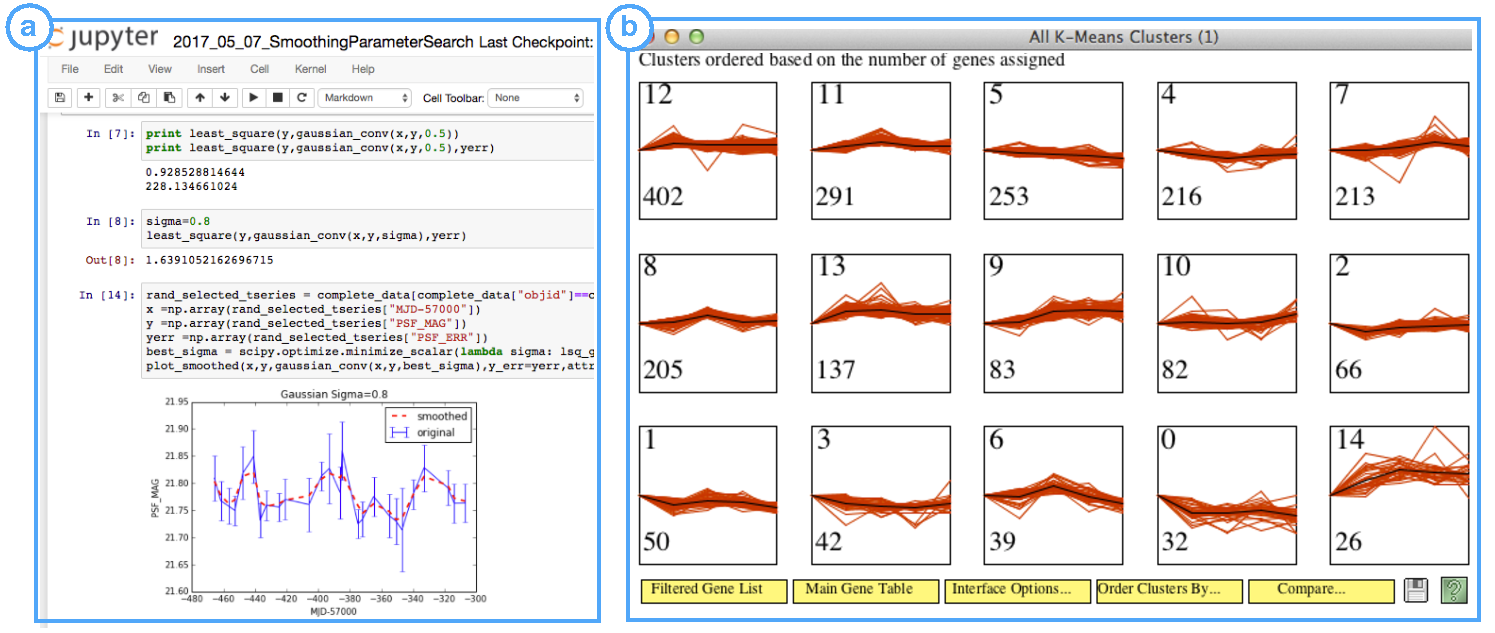
\includegraphics[width=\linewidth]{figures/workflow.pdf}
		\caption{Examples of the scientists' original workflow: a) The astronomer performs various data analysis task using the Jupyter notebook environment, b) The geneticists uses a domain-specific software to examine clustering outputs.}
		\label{workflow}
	\end{figure}
}
\par \textbf{Astronomy:} Since astronomical datasets are often terabytes in scale, they are often processed and stored in highly specialized data management centers in supercomputing centers. The collaboration's data management team has created a command-line interface that enables users to easily query, browse, and download their data\techreport{\footnote{ \url{github.com/mgckind/easyaccess}}}. 
After the data is downloaded, most of the work is done programmatically through Python in an interactive Jupyter notebook environment\footnote{\url{jupyter.org}}. The astronomer inspects the data schema, performs data cleaning and  wrangling, computes relevant statistics, and generates visualizations to search for anomalies or objects of interest, as shown in Figure \ref{workflow}a.
\par While an experienced astronomer who has examined many transient light curves can often distinguish an interesting transient object from noise by sight, they must visually examine and iterate through large numbers of visualizations of candidate objects. Manual searching is time-consuming and error prone as the majority of the objects will not be astronomical transients.
Participant A1 was interested in \zv as he recognized how specific pattern queries could help scientists directly search for these rare objects. 
\techreport{\par If an object of interest or region is identified through the visual analysis, then the astronomer may be interested in inspecting the image of the region for cross-checking that the significant change in brightness of the object is not due to an imaging artifact. This could be done using a custom built web-interface that facilitates the access of cutout images for a queried region of the sky.} 

\par \textbf{Genetics:} Participant G1 processes the raw microarray data by using a preprocessing script written in R \techreport{, where she (i) sub-selects 144 genes of interest, (ii) cleans up an experimental artifact due to measurements on multiple probes, (iii) log-transforms the raw data to show a more distinct shape profile for clustering, (iv) normalizes the gene expression values into the range of 0 to 1, and (v) performs Loess smoothing with default parameters to reduce the noise in the data}. To analyze the data, the preprocessed data is loaded into a desktop application for visualizing and clustering gene expression data\footnote{ \url{www.cs.cmu.edu/~jernst/stem/}}. G1 sets several clustering and visualization parameters on the interface before pressing a button to execute the clustering algorithm. The cluster visualizations are then displayed as overlaid time series for each cluster, as shown in the visualization in Figure \ref{workflow}b. G1 visually inspects that all the patterns in each cluster look ``clean'' and checks the number of outlier genes that do not fall into any of the clusters.  If the number of outliers is high or the visualizations look unclean, she reruns the clustering by increasing the number of clusters. Once the visualized clusters look ``good enough'', G1 exports the cluster patterns into a csv file to be used as features in their downstream regression tasks.
\par Prior to the study, the student (G1) and PI (G3) spent over a month attempting to determine the best number of clusters for their upstream analysis based on a series of static visualizations and statistics computed after clustering. While regenerating their results took no more than 15 minutes every time they made a change, the multi-step, segmented workflow meant that all changes had to be done offline, so that valuable meeting time was not wasted trying to regenerate results. The team had a vested interest in participating in the design of \zv as they saw how the interactive nature of VQSs and the ability to query other time series with clustering results could dramatically speed up their collaborative analysis process. 
\par \textbf{Material Science:} Participant M1 starts his data exploration process with a list of known and proven solvents as a reference. For instance, he would search for solvents which have boiling point over 300 Kelvins and the lithium solvation energy under 10 kcal/mol using basic SQL queries. This would help him narrow down the list of solvents, and he would continue this process with other properties. The scientist also considers the availability and the cost of the solvents while exploring the dataset. When the remaining list of the solvents is sufficiently small, he drills down to more detail (e.g., such as looking at the chemical structure of the solvents to consider the feasibility of conducting experiments with the solvent). While he had identified potential solvents through  manual lookup and comparison,  the process lacked the ability to reveal complicated trends and patterns that might be hidden, such as how the change in one attribute can affect the behavior of other attributes of a solvent. M1 was interested in using a VQS as it was infeasible for him to manually compare between large numbers of solvents and their associated properties manually.
\raggedbottom
%!TEX root = main.tex
\begin{figure*}[ht!]
\centering
\vspace{-15pt}
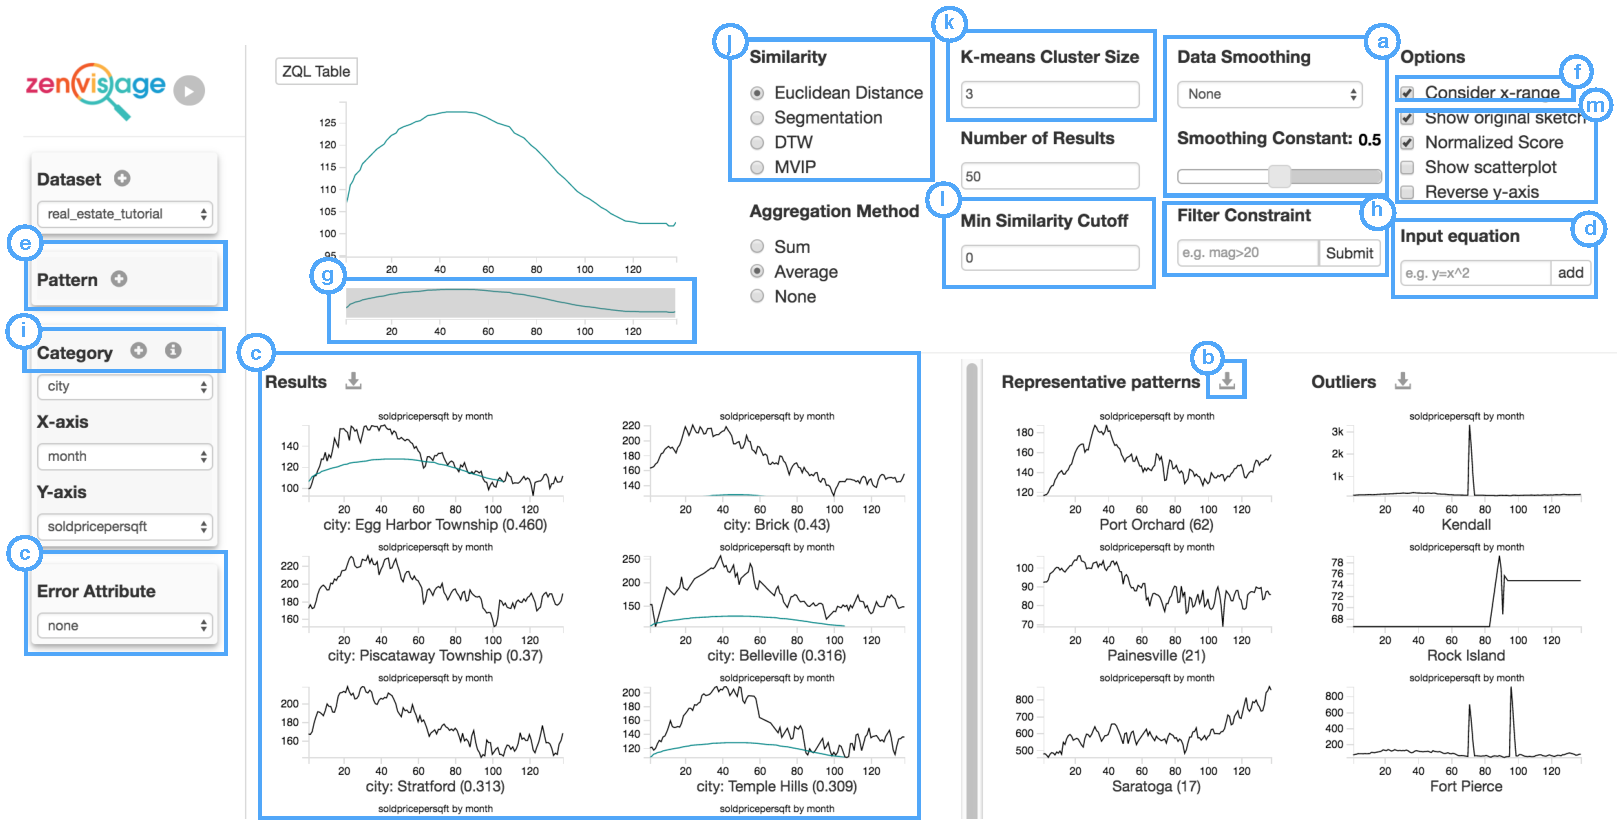
\includegraphics[width=\linewidth]{figures/newZV.pdf} %5.5
\vspace{-5pt}\caption{Our VQS after participatory design, which includes: the ability to preprocess via (a) interactive smoothing; (b, c) the ability to export data outputs ; querying functionalities via (d) equations and (e) patterns; query specification mechanisms including (f) x-range invariance, (g) x-range selection and filtering, (h) Filtering, and (i) Dynamic class creation; (j, k, l) system parameter options; (m) visualization display options. Prior to the participatory design, \zv only included a single sketch input with no additional options. \zv also displayed representative patterns and outlier patterns, as shown in Figure~\ref{oldZV}.}
\label{zvOverview}
\vspace{-14pt}
\end{figure*}

\section{Themes Emerging from Participatory Design (RQ2)}\label{findings}
\par In the previous section, we gained an understanding of the current analysis workflows employed in the three use cases. Next, to address RQ2, we employed participatory design with our scientists to incorporate key features  missing in our original VQS, and unaddressed in their
current workflows. We discovered three central themes encapsulating these features that are important to facilitate rapid hypothesis generation and insight discovery, but are missing in prior VQSs,  described next. While some of our findings echo prior work on system-level taxonomies of visualization tasks \cite{Amar2005,Heer2012}, we highlight how specific analytic tasks and interaction features could be used to enhance VQSs in particular. \techreport{In particular, we learned that \textit{participants wanted more control over the internals of the systems and an integrated workflow that helped streamline their analysis when using VQSs.}}
\subsection{Uninterrupted workflow}
\par Our cognitive walkthroughs revealed that in many participants' existing workflows, they switched between parameter specification, code execution, and visualization comparisons. The non-interactive nature of these segmented workflows has been shown to incur a large cognitive barrier during exploratory data analysis \cite{Kery2017}. In addition, since scientific research often takes place in a collaborative setting, this means that the data sense-making process could be delayed by weeks because the analysis-to-results phases needed to be rerun offline based on changes that were suggested during a meeting. Moreover, data-cleaning emerged as a common pain-point, echoing prior work~\cite{kandel2012profiler,Guo2011}.

%%%%%%%%%%%%%%%%%%%%%%%%%%%%%%%%%

\stitle{Integrative preprocessing through interactive smoothing:} While \zv does not attempt to solve all of the pre-processing issues that we faced during participatory design, we identified that data smoothing is a common data cleaning procedure~\cite{simonoff2012smoothing} that would benefit from a tight integration between pre-processing and visual analysis.  
\tvcg{\par Data smoothing is a denoising procedure that generates a smoothed pattern approximating key features of the visualized trend with less noise. Smoothing also raises an interesting trade-off between the smoothness of the curve and the quality of shape-matching for VQSs. If the visualization is over-smoothed, then shape matching would return results that only loosely resemble the query pattern. However, if no smoothing is applied, then the noise may dominate the overall trend, which could also lead to bad pattern matches. In addition, it is often hard to tell what the appropriate smoothing parameter should be applied simply by visualizing a small number of sampled visualization, as one would do in an offline analysis.}
%\kk{We don't need to define this -- a citation would suffice.} %\dor{I think this paragraph is important to keep to reflect why smoothing is not a one-shot operation and how it works with the querying functionalities of the system, perhaps need to shorten this.}}
\par To address this issue, we developed an interface for users to interactively adjust the data smoothing algorithm and parameters on-the-fly to update the resulting visualizations accordingly (Figure \ref{zvOverview}a). This was applied to the \matsci and \astro use cases, as both had noisy and dense observational data. 

%%%%%%%%%%%%%%%%%%%%%%%%%%%%%%%%%
\stitle{Facilitating export for downstream analysis:} Since \tvcg{VQSs are designed to be exploratory tools that suggest potential directions for further analysis, rather than for performing one-shot operations, we asked participants how they envisioned themselves using VQSs in their workflow}. Both the \astro and \bio participants wanted to use VQSs as a way to identify interesting objects or characteristic patterns, which they will later feed into a more advanced downstream pipeline. 
\par To smoothen the transition between the VQS and their downstream analysis, we implemented export functionalities for downloading the similarity, representative trend and outlier results as csv files (Figure \ref{zvOverview}b). Individual visualizations can also be downloaded by double-clicking individual figures(Figure \ref{zvOverview}c) to facilitate easier sharing of visualization results with collaborators. 
%%%%%%%%%%%%%%%%%%%%%%%%%%%%%%%%%%%%%%%%%%%%%%%%%%%%%%%%%%%%%%%%%%%%%%%%%%%%%%%%%%%%%%%%%%%%%%%%%%%% 
%\subsection{Sophisticated data operations in a VQS}
\tvcg{\subsection{Increasing expressiveness of querying capabilities}}
%%%%%%%%%%%%%%%%%%%%%%%%%%%%%%%%%
The initial VQS did not satisfy the participants' needs for sophisticated data operations. They wanted more expressive ways to explore their data, either through additional querying methods, or the ability to query on a subset of data.
\par While the interactions in our original system enables simple queries, many scientists were interested in extending their querying capabilities, either through different modalities of querying or through more flexible query expression.  

\stitle{Input Equations:} Our \matsci participants expressed that some solvents can have analytical models that characterize the relationships between chemical properties. They wanted to find solvents that satisfied these relationships. We implemented a feature that plots a given function (e.g. $y=x^2$) on the canvas, which is then used as input for similarity search (Figure \ref{zvOverview}d).

\stitle{Upload Pattern as Query:} While the input equation is useful when simple analytical models exist, this may not be true for other domains. In these cases, users can upload a query pattern of a sequence of points (Figure \ref{zvOverview}e). This is useful for patterns generated from advanced computational models used for understanding scientific processes, usually as part of the downstream analysis of the exploratory workflow. %For example, the \bio team are trying to develop a time series prediction algorithm using machine learning based on some biological parameters \cite{Peng2016}. For the \astro team, it is also common to compare synthetic light curves generated from simulations against observations \cite{Nugent1997}.
\stitle{Consider/Ignore x-range:} We improved query specification by allowing users to change how the shape-matching criterion is applied. For finding supernovae, A1 primarily cared about the existence of a peak above a certain amplitude with an appropriate width of the curve, rather than the exact time that the event occurred, leading them to use the consider x-range feature (Figure \ref{zvOverview}f). G1 also expressed that she does not really know what is the ``trigger point'' of when the expression level of a gene will rise and it would be interesting to find all ``rising'' profiles independent of the change-point.  We implemented an option to ignore the x-range in shape matching and a brushing mechanism that enables users to select the specific x-region they want to perform their shape matching on (Figure \ref{zvOverview}g). 
%%%%%%%%%%%%%%%%%%%%%%%%%%%%%%%%%
\subsection{Ability to dynamically facet through subsets}
\par Past studies in taxonomies of visualization tasks have shown that it is important to design features that enable users to select relevant subsets of data in visual analytics\cite{Amar2005,Heer2012}. We designed two dynamic faceting features coupled with coordinated views that enabled users to specify subsets of data they are querying on and see immediate changes updated in the query, representative, and outlier results. 

\stitle{Filtering Constraints:} Users with large datasets first used their domain knowledge to narrow down their search to a subset of data. This would increase their chances of finding an interesting pattern for a given query. To enable filtering of data, users could submit one or more SQL-like \texttt{WHERE} conditions as filter constraints in a text field (Figure \ref{zvOverview}h). \ccut{The filtering can be done on data columns associated with each pattern that is not visualized or on the visualized attributes.} 

\stitle{Dynamic Class Creation:} In order to address the material scientists' needs for creating subsets (or classes) of data on-the-fly to make comparisons between them, we implemented dynamic class creation. This feature allows users to bucket data points into customized classes based on existing properties, and subsequently allows users to compare between the customized classes. For example, the scientists can create three different classes based on a single property alone: Solvents with ionization potential under -10 kJ/mol, over -8 kJ/mol, and ones that fall between -10 and -8 kJ/mol. Then, they could browse how the lithium solvation energy differed for the the three custom classes. 
\par Scientists can utilize multiple properties to create custom classes, effectively slicing-and-dicing the data based on their needs. The information regarding the created classes is displayed in the dynamic class information table or as a tooltip over the aggregated visualizations\tvcg{, as shown in Figure~\ref{dcc}.}
\begin{figure}[ht!]
\centering
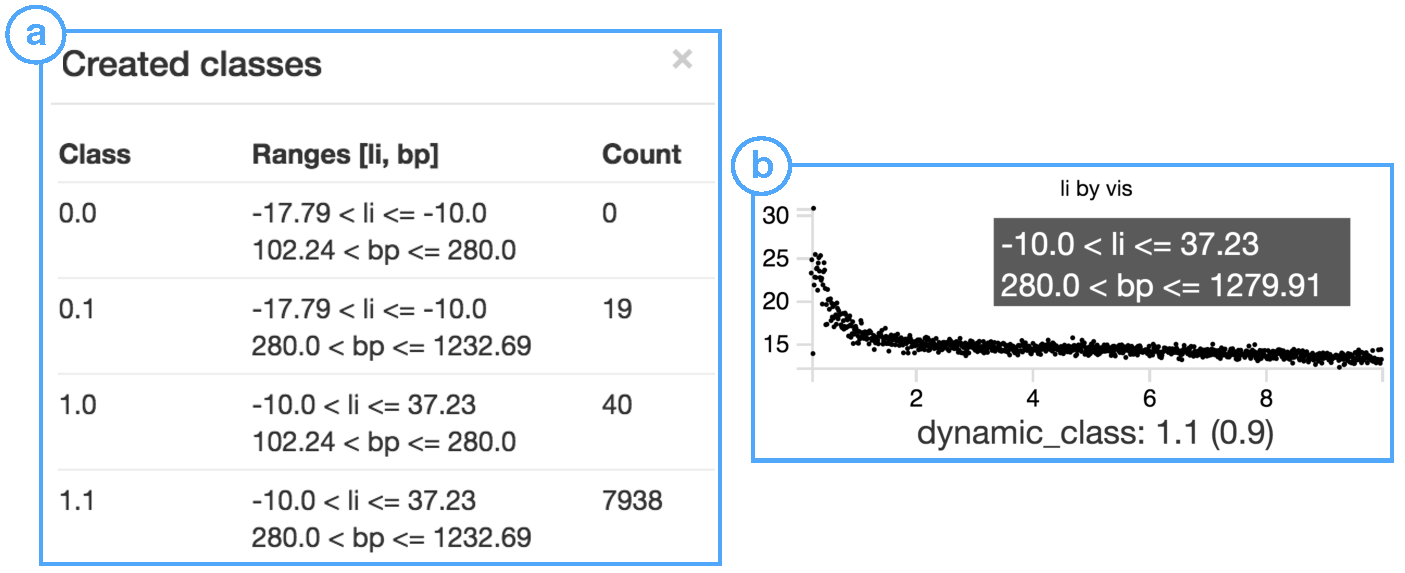
\includegraphics[width=\linewidth]{figures/dcc_example.pdf}
\vspace{-6pt}
\caption{Example of dynamic classes. (a) Four different classes with different Lithium solvation energies (li) and boiling point (bp) attributes based on user-defined data ranges. (b) Users can hover over the visualizations for each dynamic class to see the corresponding attribute ranges for each class. The visualizations of dynamic classes are aggregate across all the visualizations that lie in that class based on the user-selected aggregation method.}
\label{dcc}
\end{figure}
%%%%%%%%%%%%%%%%%%%%%%%%%%%%%%%%%
\subsection{Finer System-level Control and  Understanding}
\par During the participatory design exercise, we found that many of the features suggested by the participants indicated they wanted finer control of the system. Prior work in direct manipulation visual interfaces has suggested that finer-grained control enabled users to discover patterns and rapidly generate hypothesis based on visual feedback \cite{Shneiderman1994,Shneiderman2007a}. 
<<<<<<< HEAD

\stitle{\tvcg{Controlling VQS internals:}}
In addition to query and dataset specifications, users also wanted the ability to modify the model parameters in \zv. Our findings echoed Chuang et al.~\cite{Chuang2012}, which showed that the ability to modify the model can facilitate interpretation and trust in model-driven visualizations, especially during early-stage exploration. These model parameter options include the ability to change the choice of similarity metrics (Figure \ref{zvOverview}j), the cluster size in the representative patterns (Figure \ref{zvOverview}k), setting a minimum similarity threshold for displaying the search results (Figure \ref{zvOverview}l), and the ability to tune the smoothing algorithm and parameter (Figure \ref{zvOverview}a).

\stitle{\tvcg{Displaying interpretable explanations for VQS recommendations:}} 
Explanatory system outputs include displaying similarity scores of the outputs, the number of datapoints in each cluster, and overlaying the original query sketch on the return visualization for comparison (Figure \ref{zvOverview}m). We further provided display-related options for plotting modifications, including displaying error bars, and toggling between a scatterplot and line chart view, to help analysts better understand the visualizations.
=======
\par \textbf{\tvcg{Controlling VQS internals:}}
In addition to query and dataset specifications, users also wanted the ability to modify the model parameters in \zv. Our findings echoed Chuang et al.~\cite{Chuang2012}, which showed that the ability to modify the model can facilitate interpretation and trust in model-driven visualizations, especially during early-stage exploration. These model parameter options include the ability to change the choice of similarity metrics (Figure \ref{zvOverview}f), the cluster size in the representative patterns (Figure \ref{zvOverview}g), setting a minimum similarity threshold for displaying the search results (Figure \ref{zvOverview}h), and the ability to tune the smoothing algorithm and parameter (Figure \ref{zvOverview}i).
\par \textbf{\tvcg{Displaying interpretable explanation for why VQS recommended particular visualizations:}} 
Explanatory system outputs include displaying similarity scores of the outputs, the number of datapoints in each cluster, and overlaying the original query sketch on the return visualization for comparison. We further provided display-related options for plotting modifications, including displaying error bars, and toggling between a scatterplot and line chart view, to help analysts better understand the visualizations.
>>>>>>> 08008e20f4a35ad4452ebd11a770d0540d87e261
%\cut{, and reversing the y-axis.} 
%%%%%%%%%%%%%%%%%%%%%%%%%%%%%%%%%%%%%%%%%%%%%%%%%%%%%%%%%%%%%%%%%%%%%%%%%%%%%%%%%%%%%%%%%%%%%%%%%%%%%
%!TEX root = main.tex
\section{Final Evaluation Study: Methodology and Results} \label{evaluation}
\par Our final evaluation study addresses RQ3 and 4---whether our new and improved VQS helps accelerate insight, and how it could fit into real analysis workflows. Participants for the evaluation study were recruited from each of the three aforementioned research groups. Prior to the study, we asked the potential participants to fill out a pre-study survey to determine their eligibility. Eligibility criteria included: being an active researcher in the subject area with more than one year of research experience, and having worked on a research project involving data of the same nature as that used in the participatory design. Four of the user studies were conducted remotely.  
\par Participants had the option of exploring their own dataset or an existing dataset that they provided to us during the participatory design process. All three blank-slate participants opted to explore their own datasets. After loading their dataset, we emailed them a screenshot of a visualization from our tool to verify that we configured the system to meet their needs. 
\par At the start, participants were provided with an interactive walk-through explaining the details of the features offered in our VQS. The participants were then given approximately ten minutes to experience a guided exploration of our VQS with a preloaded real-estate example dataset from Zillow \cite{zillow}. \techreport{This dataset contained housing data for various cities, metropolitan areas, and states in the U.S. from 2004-15.} After familiarizing themselves with the tool, we loaded the participant's dataset and suggested an appropriate choice of axis to begin the exploration. Participants were encouraged to talk-aloud during the data exploration phase.
\par During the exploration phase, participants were informed that they could use other tools as needed. If the participant was out of ideas\ccut{ for three minutes}, we suggested one of the ten main operations\footnote{query by sketching, drag-and-drop, pattern loading, input equations, representative and outliers, narrow/ignore x-range options, filtering, data smoothing, creating dynamic classes,  data export} that they had not yet covered. If any of these operations were not applicable to their specific dataset, they were allowed to skip the operation after having considered how it may or may not be applicable to their workflow. The user study ended after they covered all ten main functionalities. On average, the main exploration phase lasted for 63 minutes. After the study, we asked them open-ended questions about their experience. 
%%%%%%%%%%%%%%%%%%%%%%%%%%%%%%%
\subsection{Data Collection \& Analysis}
We recorded audio, video screen captures, and click-stream logs of the participant's actions during the evaluation study. We analyzed the transcriptions of these recordings \tvcg{through open-coding and
categorized every event in the user study using the coding labels:} 
\begin{denselist}
    \item Insight (Science) \textbf{[IS]}: Insight that connected back to the science (e.g. ``This cluster resembles a repressed gene.'')
    \item Insight (Data) \textbf{[ID]}: Data-related insights (e.g. ``A bug in my data cleaning code generated this peak artifact.'')
    \item Provoke (Science) \textbf{[PS]}: Interactions or observations made while using the VQS that provoked a scientific hypothesis to be generated.
    \item Provoke (Data) \textbf{[PD]}: Interactions or observations made while using the VQS that provoked further data actions to continue the investigation.
    \item Confusion \textbf{[C]}: Participants were confused during this part of the analysis.
    \item Want \textbf{[W]}: Additional features that participant wants, which is not currently available on the system.
    \item External Tools \textbf{[E]}: The use of external tools outside of \zv to complement the analysis process.
\end{denselist}
\par In addition, \tvcg{based on the usage of each feature during the user study, we categorized each of the features into one of the three usage types:} 
\begin{denselist}
    \item Practical usage \textbf{[P]}: Features used in a sensible and meaningful way during user study.
    \item Envisioned usage \textbf{[E]}: Features which could be used practically if the envisioned data was available or if they conducted downstream analysis, but was not performed due to limited time during the user study. 
    \item \tvcg{Not useful \textbf{[N]}: Features that are not useful or do not make sense for the participant's research question and dataset.}
\end{denselist}
\tvcg{We chose to derive these labels from the user study transcription rather than through self-reporting to circumvent the bias that users may have when self-reporting, which can often artificially inflate the usefulness of the feature or tool under examination.} %\dor{Added based on Hidy's feedback.}}

\begin{figure}[ht!]
    \centering
    \vspace{-10pt}
    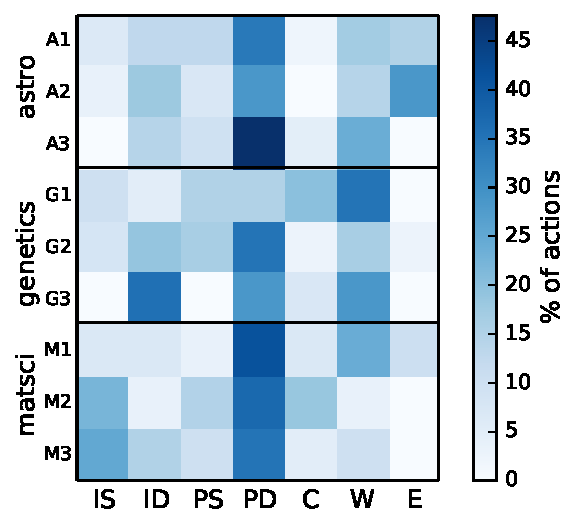
\includegraphics[width=0.7\columnwidth]{figures/result1.pdf}
    \vspace{-6pt}\caption{Heatmap \tvcg{showing percentage of participants' actions on \zv falling under each thematic encoding category.} \zv provokes participants to perform many data actions \textbf{[PD]} and generate scientific hypothesis \textbf{[PS]}. Occasionally, the series of data operations and hypothesis can lead to an scientific \textbf{[IS]} or data-related insight \textbf{[ID]}.}
    \vspace{-10pt}
    \label{action_heatmap}
\end{figure} 

\begin{figure}[ht!]
    \centering
    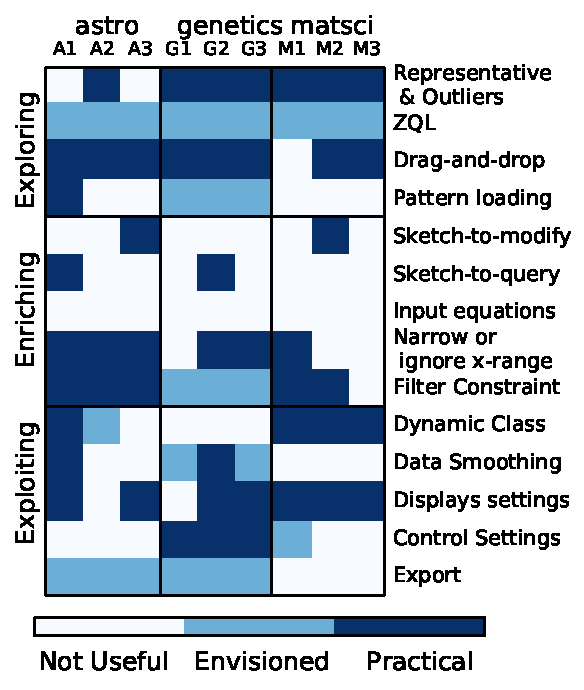
\includegraphics[width=0.7\columnwidth]{figures/result2.pdf}
    \vspace{-6pt}\caption{Heatmap of features that have a practical usage (P), envisioned usage (E), and \tvcg{not useful} (N). We find that participants preferred to query using bottom-up methods such as drag-and-drop over top-down approaches such as sketching or input equations. Participants found that data faceting via filter constraints and dynamic class creation were powerful ways to compare between subgroups or filtered subsets. The columns are arranged in the order of subject areas and the features are arranged in the order of the three foraging acts.}
    \label{feature_heatmap}
    \vspace{-5pt}
\end{figure}

\par \tvcg{The audio recordings and transcriptions of pre- and post-study interview questions are thematically encoded and summarized in Figure \ref{action_heatmap} and \ref{feature_heatmap}. }%\tvcg{The audio recordings and transcriptions of pre- and post-study interview questions revealed how \ourVQS differed from the scientist's original workflow, how they envisioned the VQS fit into their workflow, and  the pros and cons of the system. The results based on this thematic coding is depicted in Figure \ref{action_heatmap} and \ref{feature_heatmap}.}\cut{, and will be discussed in the next section.}
%\tvcg{We now describe our study results for RQ3 (how VQS features were used in practice to achieve scientific insights) and RQ4 (where VQSs fit into real data analysis workflows).} 
\tvcg{Our study results fall into two main themes, which will be discussed in subsequent sections. First, we discuss how VQS features were used in practice to achieve scientific insights (RQ3). We find that VQSs can enable rapid, fluid iteration, catalyzing new questions or insights; that different querying modalities in VQSs supported different forms of exploration; and that expressive querying allowed participants to compose novel analysis patterns. Second, we determine where VQSs fit into real data analysis workflows (RQ4). We find that VQSs can be used for a range of tasks that go beyond just exploration; that participants used the outputs from VQSs in various ways; and that VQSs are most appropriate for certain types of datasets.}

%!TEX root = main.tex
\section{Actionable VQS features for scientific insight (RQ3)} \label{VQS_features_discussion}
\tvcg{\subsection{Top-down v.s. Bottom-up analysis}}
To contextualize our study results with respect to prior work on how analysts make sense of data, we employ Pirolli and Card's~\cite{Pirolli} information foraging framework for domain-experts. Pirolli and Card's notional model distinguishes between information processing tasks that are \textit{top-down} \cut{(from theory to data)} and \textit{bottom-up} \cut{(from data to theory)}. \tvcg{Recent work in have also used the top-down v.s. bottom-up framework in understanding visualization construction\cite{Mendez2017}. In the context of visualization querying, top-down approaches are attribute-level specification to a query or an action, whereas bottom-up approaches originates from the data (or equivalently, the visualization).} 
\tvcg{\subsubsection{Querying Behavior}}
\par Our interactions with the scientists showed that different modalities for inputting a query can be useful for different problem contexts. \tvcg{To our surprise, despite the prevalence of sketch-to-query systems in literature, only two out of our nine users had a practical usage for query by sketching.} Overall, \tvcg{we found that} bottom-up querying via drag-and-drop was more intuitive and commonly used than top-down querying \tvcg{methods, such as} sketching or input equations. 
\par The main reasons why participants did not find sketching useful was that they often do not start off their analysis with a pattern in mind. Later, their intuition about what to query is derived from other visualizations that they see in the VQS, in which case it made more sense to query using those visualizations as examples directly (via drag-and-drop). In addition, even if a user has a query pattern in mind, sketch queries can be ambiguous \cite{correll2016semantics} or impossible to draw by sketching (e.g. A2 looked for a highly-varying signal enveloped by a sinusoidal pattern indicating planetary rotation). 
\tvcg{\par The latter case is also evident from the unexpected use cases where sketching was simply used as a mechanism to modify the drag-and-dropped queries. As shown in Figure \ref{query_modification} top, M2 first sketched a pattern to find solvent classes with anticorrelated properties. However, the sketched query did not return the visualization he was interested in. So, he instead dragged and dropped one of the peripheral visualizations that was close enough to his desired visualization to the sketchpad and then smoothed out the noise due to outliers datapoints by tracing a sketch over the visualization. M2 repeated this workflow twice in separate occurrences during the study and was able to derive insights from the results. Likewise, A3 was interested in pulsating stars characterized by dramatic changes in amplitudes in the light curves. During the search, hotspots on stellar surfaces often show up as false positives as they also result in dramatic amplitude fluctuations, but happen at a regular interval. On the VQS, A3 looked for patterns that exhibits amplitude variations, but also some irregularities. As shown in Figure \ref{query_modification} bottom, she first picked out a regular pattern (suspected star spot), then modified it slightly so that the pattern looks more irregular. 
\begin{figure}[ht!]
    \centering
    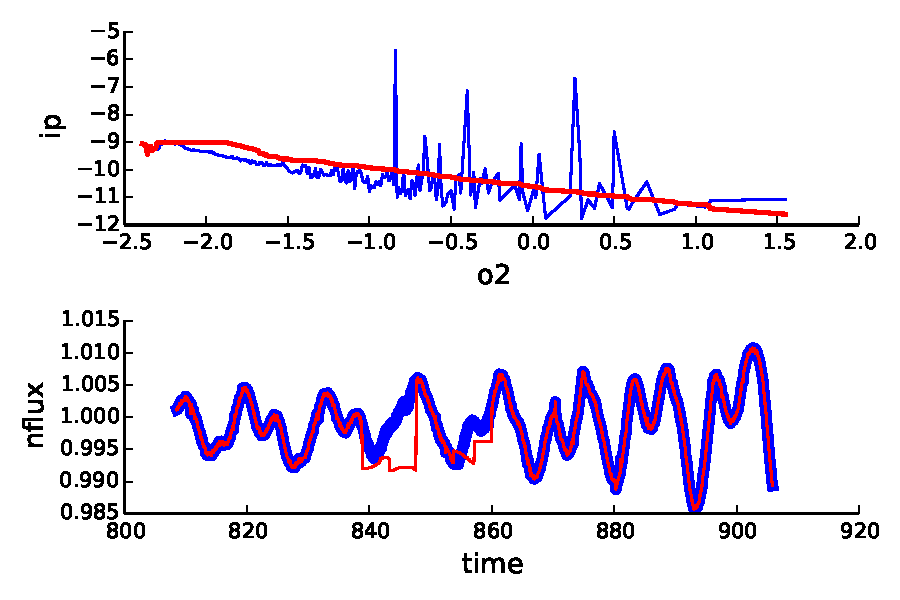
\includegraphics[width=\columnwidth]{figures/QueryModificationBySketch.pdf}
    \caption{\tvcg{Examples of query modification by M2 (top) and A3 (bottom) performed during the study The inital drag-and-dropped query is shown in blue and the sketch-modified queries is shown in red.}
    \label{query_modification}}
\end{figure}
\par Both of these use cases suggest that while sketching is an useful analogy for people to express their queries, the existing ad-hoc, sketch-only model for visualization querying is insufficient without data examples that can help analyst jumpstart their exploration. \emph{We suspect that this is why existing sketch-to-query systems are not commonly adopted in practice despite extensive research. This result, however, points to a potential need for high-level query modification interfaces that enable more precise visualization query specification in future VQSs.}} %This, however, points to an exciting direction for sketching interface in VQSs for developing advanced drawing and modification tools that enable more precise visualization query specification.}
\par Despite functional fitting being common in scientific data analysis, Figure \ref{feature_heatmap} shows that querying by equation is also unpopular for the same reason as a sketched query. In addition, the visualizations for both \astro and \bio exhibit complex processes that could not be written down \tvcg{as an equation} analytically. However, even when analytical relationships do exist (in the case of \matsci), it is challenging to formulate functional forms in an \tvcg{prescriptive,} ad-hoc manner. %For instance, \matsci discovered a known inverse relationship during exploration
%Which is really interesting. Which is something that we observed experimentally also. That is an interesting insight right htere. This seems to suggest that there is a fundamental issue in if you want to try to get better on this axis, and get as low as possible, you lose out on the other axis.
%once they see it they know it but they don't know beforehand
\par \tvcg{In contrast, when we looked at bottom-up querying approaches}, drag-and-drop was the querying mechanism used most frequently by the participants. Examples of practical uses of drag-and-drop includes inspecting the top-most similar visualizations that lie in a cluster and finding visualizations that are similar to an object of interest that exhibits the desired pattern. \tvcg{Likewise,} many participants envisioned use cases for pattern loading. \tvcg{The ability to load in data patterns as a query would enable users to compare} visualizations between different experiments, species, or surveys, querying with known patterns from an external reference catalog (e.g. important genes of interest, objects labeled as supernovae) \tvcg{or verify} the results of a simulation or downstream analysis by finding similar patterns in their existing dataset. \tvcg{In addition, users can also specify} a more precise query that captures \tvcg{the essential shape features of a desired pattern} (e.g. amplitude, width of peak), which can not be precisely drawn as a sketched pattern. \tvcg{For example, as shown in the top left diagram in Figure \ref{example}, the width of the light curve is characteristic to the type of supernovae that its associated with and is therefore helpful for distinguishing the queried pattern from noise.}
\par While the usage of each querying feature may vary from one participant to the next, generally,  drag-and-drop and pattern upload are considered bottom-up approaches that go from data to theory by enabling users to query via examples of known visualizations. For top-down approaches such as query by sketching and input equations, the user starts with \tvcg{an intuition about how their desired patterns should look like based on theory, then queries based on that}. Our results indicate that \emph{bottom-up querying approaches are preferred over top-down when the users have no desired patterns in mind}, which is commonly the case for exploratory data analysis.
% \paragraph{Both top-down and bottom-up faceted exploration enable users to derive insights through VQSs.} 
%\subsection{Top-down and bottom-up faceted exploration} 
\tvcg{\subsubsection{Faceted Exploration Behavior}}
\par All participants either envisioned a use case or utilized \tvcg{the data faceting functionalities offered in \zv (filtering,  dynamic class)} to explore and compare subsets of their data. 
\par A1 expressed that even though the filtering step could be easily done programmatically on the dataset and reloaded into \zv, the filter constraint was a powerful way to dynamically test their hypothesis. Interactive filtering lowers the barrier between the iterative hypothesis-then-compare cycle, thereby enabling participants to test conditions and tune values that they would not have otherwise modified as much.
% echoing our previous finding that segmented workflow prevents extensive exploration.
During the study, participants used filtering to address questions such as: ``Are there more genes similar to a known activator when we subselect only the differentially expressed genes (e.g. DIFFEXP=1)?'' (G2) or ``Can I find more supernovae candidates if I query only on objects that are bright and classified as a star (e.g. flux\textgreater
10 AND CLASS\_STAR=1)?'' (A1). Three participants had also used filtering as a way to pick out individual objects of interest to query with. For example, G2 set the filter as gene=`9687' and explained \tvcg{that because ``
this gene is regulated by the estrogen receptor, when we search for other genes that resembles this gene, we can find other genes that are potentially affected by the same factors.''}
As shown in Figures \ref{action_heatmap} and \ref{feature_heatmap}, participants with the top-most provoked data actions (A1, A3, G2) made heavy use of filtering to explore different subsets of the data. 
\par While filtering enabled users to narrow down to a selected data subset, dynamic class creation enabled users to compare the relationships between multiple physical attributes and between subgroups of data. For example, M2 divided the solvents in the database to eight different classes based on the voltage properties, state of matter at room temperature, and viscosity levels, by dynamically setting the cutoff values to create these classes. By exploring the created custom classes, M2 learned that the relationship between viscosity and lithium solvation energy is independent of whether a solvent belongs to the class of high voltage or low voltage solvents. M2 cited that dynamic class creation was central to learning about this previously-unknown property of these two attributes: 
\begin{quote}
All this is really possible because of dynamic class creation, so this allows you to bucket your intuition and put that together. [...] I can now bucket things as high voltage stable, liquid stable, viscous, or not viscous and start doing this classification quickly and start to explore trends. [...] And look how quickly we can do it! Quite good!
\end{quote}
\par Participants employed \emph{a mix of bottom-up and top-down approaches when faceting through data in VQS}, including narrowing the search space based on some intuition about a phenomena, selecting individual visualizations, or specifying high-level groupings to compare and query with.
%selectively finding high-level grouping to compare and query with
% This was a finding that M2 have not previously One participant discovered that certain physical properties were decoupled from the high voltage properties of solvents. ``These properties are decoupled from the high voltage properties which is something that makes a whole lot of sense.'' When asked if he knew of this fact, he replied  ``Probably not. I mean I could have guessed. But [...] I would not have conclusively said that this is obvious.'' The same participant voluntarily described this feature in his own word:
% Simmilarly, on two different ----- radius of ---, be
% bright objects and -----. 
% Dynamic classes enabled 
% \par For a similar reason, cold-start problem is difficult for top-down approaches. input equations as query was an unpopular choice since both astronomy and biology had complex processes that could not be written down analytically. Only one of our participant used it ---, fammilar with functional fitting 
% this was surprising as functional fitting is a common procedure conducted in scientific analysis, but it is not suited for querying a visualization. 
% \par  \textbf{Cold-start problem:}
% One of the ---- coming up with what to query 
% In the control panels, --- however, Novices often don't have an idea of what to try 
% Interaction wise some participants wanted ----, 
% instruction manual showcasing examples of when and how each data ---- should be used. 

% peripheral viewing of visualization ----
% Another ----- , cold-start problem --- multiples of visualizations provided a way for ----- cold start problem. a lot of learning happening if this is a new dataset. All of except one our users have found outliers 
% (the last user used the results pane to scroll through and browse data with the default query)
% 2 out of the 5 datasets that participants used in the user study were preliminary dataset that had minimal data cleaning and transformations. 

% \par \textbf{Information Foraging in VQS:}

\subsubsection{Novel workflows focusing on one central foraging act.}\label{novel_workflow_foraging}
\par Pirolli and Card's notional model further characterize the trade-offs between three central activities in the information foraging process: exploring, enriching, and exploitingd~\cite{Pirolli}. \textit{Exploring} involves gathering more information during the analysis. \tvcg{In the context of VQSs}, exploring includes viewing representatives and outliers, incidental viewing of other visualizations \tvcg{in the ranked search results}, and querying via drag-and-drop and pattern-loading. \textit{Enriching} involves tasks that narrow down the space of analysis, such as filtering, dynamic class creation, query specification, and querying via input equations and sketching. \textit{Exploiting} involves spending time inspecting the results in more detail, including interpreting each visualization in greater detail or making plotting changes that offer another perspective (smoothing, display, and interpretability settings). %\dor{This paragraph was moved from beginning of Sec 6 to here, the notion of bottom up and top down is removed in this discussion to avoid confusion.}
% Given these observations on how users make use features, we discuss some of the unexpected workflows that the users have constructed to fit their use cases that made use of many features in VQS. Workflow that the participants contructed within \zv consist of ---- multiple interactions, settings ,queries , .etc that work together to a larger high-level goal. 
\par In addition to \tvcg{observing} how participants use features within \tvcg{the VQS}, we also find that participants often create unexpected workflows that chain together multiple \tvcg{analysis steps, including} interactions, controls, and queries in order to address a higher-level research question. These behaviors can be explained in terms of the foraging acts \tvcg{proposed by Piroli and Card.} We find that participants often construct a central workflow, \tvcg{which they then iterate on while adding additional variations.} \ccut{then they continue to perform the same workflow over and over with additional variations.} Their \emph{central workflow often resembles one of the three foraging acts} that aligns with the type of research question and dataset they are interested in. The variations are based on intermixing their central workflow with the other two foraging \tvcg{acts}.
% We find that participants often have a strong inclination to perform tasks that resembles one of the three foraging act and sparsely intermixed with other activities to support their analysis, depending on the type of research question and dataset they are interested in.
\par  For example, the geneticists were mostly interested in \textit{exploring} clusters to gain an overall sense what profiles exist in the dataset \tvcg{through representative trends} and therefore queried mainly through drag-and-drop. The variations to their main workflow include changing cluster sizes and display settings to offer them different perspectives on the dataset (\textit{exploit}) and filtering on data attributes (\textit{enriching}). 
%For example, G2 knew that there was three repeated measurements that was taken for every timestep, in one of the profiles there was a sharp jump whereas other datapoints are relatively flat, he then concludes by inspecting in the scatterplot view that the rise in gene expression is probably due to an experimental error rather than the activation of a gene, because the other two repeated measurements were similar in magnitude. In other words, the scatterplot view offered him density of points as another proxy to consider that was not offered in the line chart perspective.
The main workflow for the astronomers in our user study involves \textit{enriching}, either through the creation of groups or via filtering data subsets. The main workflow for \matsci involves \textit{exploiting}, since they spend the majority of their efforts performing ``close-reading'' of individual visualizations to understand the relationships between  physical variables. %This is true for both participants with and without a desired pattern in mind. For the participant without a desired pattern (G2), he created groups based on quartile statistics of additional data attributes and recorded the most significant representative pattern. 
% [---] out of 9 of our participants had more than one main workflow.
\ccut{\par Designing VQS features that diversifies potential variations and helps the creation of multiple analysis workflows that could expand the space of actions that could be performed during the analysis. Furthermore, the ability to construct these workflows within VQS relies that the users have a clear mental model for how the multiple coordinated views in the VQS interacts, as described by A2:
\begin{quote}
I like that [the VQS interface is] very clean, once you do it once or twice, you remember how this thing works. I used to know colleagues that use some software for light curve treatment and it's so full of options and suboptions that it is painful to use. In the end the software will not give you all the answers, but the analysis you made on your own.
\end{quote}
Proper explanation and documentation of the system's functionalities with examples is also crucial to help construct this mental model for how the VQS works, as G1 puts it as:
\begin{quote}
[The] features itself are good, but there should be a manual that gives examples and descriptions of each of the options and functionalities that could be done. If a person is unfamiliar with their dataset, they might not have think of which sets of operations to select, having these simple scenarios can sometimes ring a bell for them on what operations they could do. For example, when would have I do use a different similarity metric than Euclidean? When would it be good for me to view the data as a scatterplot rather than a line chart?
\end{quote}}

\tvcg{\subsection{The need for comparisons across multiple collections of visualizations on different data attributes.}}
\par All participants wanted the ability to perform comparisons across multiple collections of visualizations on different data attributes, including comparison tasks such as:
comparing between genes that belong to different functional groups (G1,G3); 
comparing between stars that harbor planets (which exhibits a transit pattern) and stars that don't (A2);
comparing similarity and dissimilarity between two different sets of y measurements, such as time series of gene expression v.s. hypersensitivity (G2), stellar fluxes across different bands (A1); and comparing the correlation between different chemical properties for different solvent groups (M2).
\par These complex tasks are akin to the queries in the Zenvisage Query Language (ZQL)~\cite{Siddiqui2017}, which we did not demonstrate to our participants during the study to avoid confusion. \tvcg{Currently, to complete these tasks using \zv},  participants would have had to use the querying interface multiple times while also remembering past results, which can be error-prone. Developing sensible interactions to map user intentions to sophisticated query languages like ZQL is an important direction for future work. 
% % Multi-group comparison could be covered by ZQL too.
% % This finding also points to the need for supporting multidimensional attribute views in VQS, 

\subsection{Integrated workflow results in more experimentation.}
\par Our participants' original workflow often requires them to compare between many visualizations manually through separate analysis and visualization steps. \ccut{The segmented analyze-then-visualize workflow is a common practice adopted by scientists who are used to thinking about visualizations as the final product of an analysis, rather than something used throughout the process to obtain insights. \cut{Since some statistical analysis can take a long time to compute, analysts often store their results separately and then visualize them with a separate module, so that ``cosmetic'' plotting changes could be applied more easily without recomputing.}} Three of the participants cited that this artificial segmentation was one of their chief bottlenecks. The cognitive overhead from the segmented workflow made them more hesitant to visualize the results of different parameters and data operations, as A2 noted:
\begin{quote}
The quick visualization is something that I could not do on my current framework. I could not query as fast as you do; I need to wait for it, plot, and then compare. Every time I plot, I need to define subplots for 12 visualizations, then its slower. That's the reason why I sometimes plot less, and I rely more on the statistics from the likelihood tests. Sometimes I plot less than I really should be doing.
\end{quote}
In Figure \ref{action_heatmap}, we also see that \zv provoked users to generate many data operations (PD) and hypotheses (PS).
\subsection{Rapid insights via VQSs catalyze new questions, hypotheses, and actions.}
\par \tvcg{The ability to rapidly experiment with large numbers of hypotheses in real time is a crucial step in the agile creative process in helping analysts discover actionable insights~\cite{Shneiderman2007a}. Five out of nine participants discussed how the dynamic, interactive update of the visualization in \zv was the main advantage for using VQSs over their original workflow.}
\par A common theme that we found across the \bio participants is that they often gain their intuition about the data from the representative trends. One example of rapid insight discovery comes from G1, G2, and G3, who first identified that the three representative patterns shown in \zv---induced genes (profiles with expression levels staying up), repressed genes (started high but went down), and transients (go up and then come down at different time points)---corresponded to the same three groups of genes discussed in a recent publication\cite{Gloss2017}. 
\par The clusters provoked G2 to generate a hypothesis regarding the properties of transients: \textit{``Is that because all the transient groups get clustered together, can I get sharp patterns that rise and ebb at different time points?''} To verify this hypothesis, G2 increased the parameter controlling the number of clusters and noticed that the cluster no longer exhibited the clean intuitive patterns he had seen earlier. G3 expressed a similar sentiment and attempted to identify different clusters. He proceeded by inspecting the visualizations in the cluster via drag-and-drop and found a group of genes that all transitioned at the same timestep, while others transitioned at different timesteps. G3 described the process of using VQSs as doing ``detective work'' that provoked him to generate further scientific hypotheses as well as data actions.
%!TEX root = main.tex
\section{VQSs within a scientific data analysis workflow (RQ4)}
\ccut{We also gained insights into how VQSs can potentially integrate with scientists' existing workflows. We start by identifying properties of ideal datasets for VQSs.}
\subsection{VQSs used beyond the exploration stage of analysis.} 
\par \techreport{Two of the five datasets used in the user study were preliminary in the sense that the scientists had performed only basic data cleaning and had not explored this dataset in great detail themselves \tvcg{(A1, G2)}. This enabled us to get a sense of how VQSs can be used in practice at different stages of the analysis workflow.} \tvcg{During the participatory design, we thought that our VQS would serve as a tool that help scientists find interesting patterns} following which scientists could proceed to a more detailed and rigorous analysis based on these newly-obtained insights. We realized after the evaluation study that users were interested in using VQSs for more than one-step pattern-finding. For example, A2 commented:
\begin{quote}
[\zv fits in] after the cleaning and after correcting for systematics, I will use \zv for a first visualization, not taking the advantage of all the features that \zv has, and then will perform a first analysis and then come back to \zv (in this analysis I will calculate the rotational period and some other values that could help me separate out the categories in \zv), then after I learn about the categories. In the end, I will again use \zv to visually inspect the data. %In stellar astronomy, visual inspection is super high rated [sic].
\end{quote}
Participants also explained where they saw VQSs fit into their workflow, including {\em (i)}
visualizing raw data before cleaning to learn about what types of outliers, representative trends, and artifacts are present in the data (A1, A2, G2, M3); {\em (ii)}
 data verification after cleaning to see if known patterns show up as expected (G1);
 and {\em (iii)}
verifying the correctness of a simulation, by visualizing data from a simulation that is based on insights obtained using the VQS (G1, G3).
\subsection{VQSs can be used for verifying data fidelity and debugging.}
\par Participants often used \zv to verify the fidelity of their data and perform debugging. For example, G2 crosschecked that there were no data artifacts of ``genes with two peaks'' via sketching.  Via the visualizations displayed in the result, representative, and outlier panels in \zv, participants were able to gain a peripheral overview of the data and spot anomalies during exploration. For example, A1 spotted time series that were too faint to look like stars after applying a filter constraint of CLASS\_STAR=1. After a series of visualizations of other query results and consultation with an external database, he concluded that the dataset had been incorrectly labelled with all the stars with CLASS\_STAR=0 as 1 during data cleaning. 
\par Explanatory display outputs \tvcg{in the VQS} work closely in conjunction with finer control mechanisms so that users receive feedback on their data actions and immediately update their mental models. For example, the genetics participants modified the clustering parameters and verified that the size of each cluster still remained relatively even, in order to determine the best values of the parameters. This served as a verification mechanism that helped users build trust in the model outputs by cross checking with their intuition on what should happen to the result as they perform an operation \cite{Chuang2012}. Moreover, the dynamic, real-time update of VQSs aid rapid hypothesis generation and encourage scientists to try things that they would not have done otherwise, especially for exploratory tasks that had a low probability of producing interesting results, such as browsing for anomalies \tvcg{as a sanity check} or data verification. 
%%%%%%%%%%%%%%%%%%%%%%%%%%%%%%%%%%%%%%%%%%%%%%%%%%%%%%%%%%%%%%%%%%%%%%%%%%%%%%%%%%%%%%%%
\subsection{VQSs are used in conjunction with external tools.}
\par During the user study, four of the scientists consulted external tools outside of the VQS as a reference. Two out of the four used the external tools to compute statistics, browse related datasets, or examine other data attributes. This shows that generic VQSs are not a one-size-fits-all solution~\cite{stonebraker2005one}, and domain-specific tools are often useful to provide context.
\techreport{\par For example, A1 saw a strange dip in the time series in the VQS and wanted to see whether it was an artifact. He first checked the database to see if there is an error flag associated with the observation of this object and learned that this object is labelled as a galaxy. Upon comparing with the other visualization in the panel in the VQS, he noticed the difference in y values and hypothesized that object was so faint that it was below the detection limit of the instrument. After going to an external software to inspect the images, he verified his hypothesis as the image was so noisy and a bright nearby star may have saturated the imaging equipment and resulting in the dip in the observations.}
\par We identified two main reason why scientists go to external tools to support their analysis in VQS. (1) Scientists often require multiple sources of data to test the validity of their hypothesis. For example, to determine whether a particular gene belongs to a regulatory network, G2 not only looks at the expression data in the VQS but also enrichment testing and knockout data. Visualizing these data often requires specialized tools and isn't  supported by a generic VQS. To enable smoother transitions between tools, several participants expressed that VQSs should bookmark and track the history of visualizations that they had found interesting. (2) Scientists also use many different data attributes to better understand the data that they are visualizing in the VQS and further develop their hypotheses. Four participants wanted the VQS to support data summaries (histograms, statistics) on the non-visualized attributes to assist them with choosing appropriate values for filtering data subsets and class creation. For instance, A2 used his Jupyter Notebook during  exploration to obtain summary statistics on radius of a star. 
\subsection{Insights derived as preliminary, and can be subjected to more robust testing or \cut{supported their intuition for more advanced }downstream modeling.}
\par We ask participants the types of additional analysis they plan to run downstream after obtaining insights from \zv. Eight out of nine participants envisioned that exporting functionalities in \zv are useful for directing them to the next step of their analysis workflow. For astronomers, the post-analysis tasks involve cross-checking and inspecting individual objects of interest more closely, including using external data types such as images. A1 discussed how he plans to perform a more rigorous ``blind analysis'', which involves taking the visualized data without any IDs or associated data attribute, and seeing if other statistical techniques yields the same set of interesting objects as the ones discovered visually through VQS. All genetics participants expressed that they will export the clusters and directly move onto the next stage of the analysis without additional verification, since they regard the results from VQS ``simply as guidelines'' (G3) that provide them with the intuition about what types of patterns exist in their dataset, before they start building advanced models. \tvcg{None of the material scientist} wanted to export their data because they were more interested in insights gained from understanding relationships between chemical properties, rather than finding particular solvents. The question of how analysts understand and trust the outputs of VQS depending on the objectives of their analysis is an interesting direction for future work.
%!TEX root = main.tex
\tvcg{\section{Reflections on Meta-analysis Methodology and Limitations}\label{metastudy}
\par Design studies are common in visualization research and often culminate in the development of a domain-specific tool, such as visualization systems for micro-array data\cite{Craig2003} or biological networks\cite{Barsky2008}. As discussed in Section~\ref{methodology_relatedwork}, unlike these design studies, most prior work in VQSs is technique-driven and is rarely evaluated on real-world users, tasks, and datasets. Prior work distinguishes between problem-driven and technique-driven research and argues that the field of visualization research benefits from contributions made from both types of methodologies\cite{Sedlmair2012,munzner2009nested}. Our work can be seen as a hybrid between problem and technique-driven work by using multiple case studies to more holistically address our research questions.%\dor{Trying to address Karrie's comment "What gap.Not evaluating on real-world task for problem-driven and technique-driven work?"} \sout{Our work seeks to bridge this gap by using multiple case studies to more holistically address our research questions.}
\par When considering a single use case study, our approach closely follows and inherits many of the benefits and pitfalls of MILCs\cite{shneiderman2006strategies}, design studies\cite{Sedlmair2012}, and insight-based evaluations\cite{North2006}. However, there are several additional pros and cons that arises when we consider our multiple case studies approach. 
%\paragraph{P1: Careful selection of case study participants results in early-stage design specification and guidelines.}

\stitle{P1: Conversation with potential collaborators establishes early-stage design specification and guidelines.} 
\npar In selecting our three user groups, we spoke to participants from 12 different potential application domains ranging from connectonomics to protein networks, in a process similar to the \textit{winnow} stage described in Sedlmair et al.\cite{Sedlmair2012}. These conversations drew us to consider what are the viable use cases for VQSs and where VQSs fail, which serves as a starting point for our design study. As a result, we distilled a set of characteristics that exemplifies use cases that may not be suitable for VQSs. We focused on the astronomy, genetics, material science groups in this paper since their data can be viewed in a line chart format and their tasks required comparisons across many visualizations. It is also important to note that selecting a diverse set of use cases in terms of the types of users, data, challenges and analysis tasks as shown in Figure \ref{example} is important for generalizing our results beyond a single use case.
\npar There were many interesting potential scientific use cases that did not satisfy these criteria. For example, time-varying 2D maps representing the interactions between brain regions and protein-protein interactions are non-ordinal heatmaps, with no simple sketching analogy. While VQSs are not restricted to only line charts, supporting querying capabilities for other visualization types is a exciting direction of future work that is outside the scope of this study. Even when the data is time series-based, some potential application domains had data characteristics that made it difficult to use a VQS. For example, a neuroscientist noted that their time series only consists of 3-5  observations, since each observation required the dissection of a mouse brain. Visualizations with sparse datapoints can be difficult for existing shape matching algorithms. \ccut{Small numbers of visualizations to compare against means that VQSs are unnecessary since manual examination may be sufficient to derive insights. \techreport{We also found that to make maximal use of \zv through faceting, their data should contain additional data columns that could support their inference.}} 
%Large, two-dimensional, and ordinal datasets are well suited for VQSs.

\stitle{P2: Parallel use case engagement results in more generalizable design and development.\notvcgTR{\footnote{While we use the term ``parallel'' in this context, since the process of design studies is highly iterative and subjective to individual participants, the progress of each case study does not have to be exactly in sync. As shown in Figure \ref{timeline}, our participatory design timeline is somewhat scaffolded.}}}
%\dor{Addressed Karrie's comment that the generalizability claim is too strong, not sure if need to tone down more.}
\npar One of the key benefits of having multiple case studies for a design study is that researchers can better evaluate a relevant set of analysis tasks to be addressed by the tool across use cases. During the design phase, researchers interact with multiple groups of participants to discuss a wide variety of problems present in their current analysis workflows and the types of tasks they want to perform on a VQS. As highlighted in Section \ref{findings}, through a series of cognitive walkthroughs and regular meetings we can distill a set of common themes that emerges across multiple use cases and rank important and relevant problems to address with the tool. Of the 20 features we implemented, 16 were suggested by multiple use cases. 
\npar For example, we spoke to astronomers who wanted to preprocess the data so that sparse time series with few numbers of observations were not included in their dataset. In the same week, we spoke to material scientists who wanted to inspect only solvents with properties above a certain threshold. Through these use cases, data filtering arose as a crucial, common operation that we needed to incorporate into \zv in order to support these class of queries.

\stitle{P3: Cross pollination of feature design leads to unexpected usage.}
\npar In addition to seeking common themes and solutions across use cases, we found that discussing newly-added features that addressed a particular use case with other groups of participants often results in unexpected usage of the feature. Continuing with the filter example, we found that participants wanted to use filter to do many types of tasks that was not originally envisioned in the design study. For example, astronomers reformatted their data and naming scheme to make use of the filter functionality to search across data of selected set of observational cycles, years, or bands. Astronomers and geneticists also used the filter operation to select specific known objects to query similar patterns. Since these unit features were inspired by multiple use cases, they cover a diverse range of foraging acts, as described Section \ref{novel_workflow_foraging}, and thereby support analysts to easily create novel analysis workflows within the VQS.

\stitle{P4: Conflicting design choices between different users results in feature generalization.}
%kk{This section is confusing}\agp{Why is this a pro?}\dor{This is good because it enables us to create more general features that can tailor to many use cases. I've modified paragraph to make this more clear.}
\npar While there are common features across use cases, we also encounter cases where variations of a feature was required or use cases that did not want a specific feature. In building a generalized tool, we opted for a default choice that was transparent to the users and a tunable option that the individual users may chose to customize. Many of the options in the systems settings panel such as data smoothing and aggregation are examples of this. For example, G1 and G2 did not want to turn on smoothing since their data was already Loess smoothed, whereas A1 was used to Gaussian Kernel smoothing. Such feature generalization enables us to create features that could be useful across multiple use cases.

\stitle{C1: Initial collaboration is time-consuming and requires significant effort.} 
\npar The process of preparing the analyst's dataset to be ready to use in our prototype tool for the design study is time-consuming. This initial phase can largely be boiled down to data requirements and system requirements. In all three of the scientific use cases, there was a period of time for establishing the minimum data and systems requirements for understanding how a VQS can be used for the particular scientific use case. Data requirements includes gaining sufficient understanding of the problem domain, understanding the types of data suitable for the system, cleaning and loading of the dataset into the tool, so that it is appropriate for use in a VQS. The minimum system requirements include features that are required for the data to be visualized appropriately, such as displaying error bars or showing the time series as scatterplots. Often, participants can only envision the types of queries that they would like to make and how finer query specifications and system controls could help better address their science questions after seeing their data displayed for the first time in the prototype system.
%Data requirements includes gaining sufficient understanding of the problem domain and dataset to help with cleaning and loading of the dataset into the tool, so that it is appropriate for use in a VQS. System requirements involves the features that are required for the analysts to understand their data within in our tool, including --- or ------. %Often the participants can only envision the types of what and how to query can only be obtained after getting over the data and system requirement.
%After seeing the data being displayed for the first time in our system according to these requirements, the scientist naturally begins to envision the types of queries that they would like to make and ways that finer query specifications and system controls that could help better address their science questions.

\stitle{C2: Failure to select the right problems and features during the design phase can result in wasted engineering efforts.}
\npar During the design phase, there were numerous problems and features proposed by participants, but not all were incorporated in the tool. Among our available meeting logs with participants, we found that the reasons for not taking a feature from the design stage to the implementation stage includes: 
\begin{denselist}
\item Nice-to-haves: One of the most common reasons for unincorporated features comes from participant's requests for nice-to-have features. The amount of nice-to-have features that one could envision for the tool is endless. We use 
two criteria to heuristically judge whether to implement a particular feature:
\begin{enumerate}[leftmargin=*]
\item \textit{Necessity:} Without this feature, can the analyst still work with this dataset using our tool and achieve what they want to do? 
\item \textit{Generality:} If this feature was implemented, will it benefit only this specific use case or be potentially useful for other applications as well?
\end{enumerate}
\item ``One-shot'' operations: We decided not to include features that were ``one-shot'' operations that only needed to be performed once during the analysis workflow. For example, certain data preprocessing operations such as filtering null values only needed to be performed once unlike the data smoothing feature that we added, which was a preprocessing step that could be iteratively performed along with other operations in the VQS. This design choice is specific to our VQS design study.
\item Substantial research or engineering effort: Some proposed features do not make sense in the context of VQS. For example, the material science group proposed functional fitting to obtain fitting coefficients. Other features requires a completely different set of research questions. For example, the question of how to properly compute similarity between time series with non-uniform number of datapoints arose in the astronomy and genetics use case, but requires the development of a novel distance metric or algorithm that is out of the scope of the RQs of our design study.
\item Underdeveloped ideas: Other feature requirements came from casual specification that were underspecified. For example, A1 wanted to look for objects that have deficiency in one band and high emission in another band, but what brightness levels qualifies as a deficiency is ambiguous.
\end{denselist}

\par Failure to identify these early signs in the design phase may result in feature implementations that turn out not to be useful for the participants. 
%(true also for single design study, but here we need to make a decision on evaluate what to build instead of simply building so that it works for a single use case.) 
Our experimental evaluation shows that some of our feature choices also suffer from these pitfalls. For example, we incorporated the feature to reverse the y-axis so that astronomers could better understand magnitude measurements (as larger magnitudes counter-intuitively corresponds to dimmer objects). In hindsight, the feature was not crucial for the analysis since another derived measure present in dataset could be selected instead and the feature was solely specific to the astronomy use case. In the end, we found that this feature was not used by any of the participants (including the proposer) in the user study.%For example, we incorporated error bars since astronomers were unable to make sense of the raw data pattern and distinguish between a real supernovae signal from fluctuations caused by noise. While we initially thought that uncertainty measurements would be a common theme across experimental data in the physical sciences, this feature was only used for the specific astronomy dataset in the study. 
}
%!TEX root = main.tex
\section{Conclusion and Future Work} \label{conclusion}
\par In the face of a data deluge in science, many scientists struggle to leverage these large datasets to derive scientific insights. While VQSs hold tremendous promise in accelerating data exploration, they are rarely used in practice. In this paper, we worked closely with three groups of scientists to learn about the challenges they face when working with data. We extended \nonannon{our VQS \zv} to the point where it could be effectively used for scientific data analysis. 
\par From cognitive walkthroughs and interviews, we learned about the challenges faced in scientific data analysis, including the lack of experimentation due to segmented workflows, and having to compare between large collections of visualizations (RQ1). Through participatory design, we identified three classes of missing interface capabilities  essential for employing VQSs for facilitating insight in real scientific applications, spanning expressive querying and dynamic faceting, as well as fine-grained control and understanding, along with the ability to compose flexible workflows in an integrated manner (RQ2). Finally, our evaluation study demonstrated how these features helped accelerate scientific insights (RQ3), as well as how they fit in the context of data analysis workflows (RQ4). One such finding is that bottom-up querying (e.g., drag-and-drop) is preferred over top-down (e.g., sketching) for exploratory data analysis, contrary to what is commonly supported in existing VQSs. Scientists were able to use \zv for debugging errors in their data, for discovering desired patterns and trends, and for obtaining scientific insights to address unanswered research questions. By extending and evaluating VQSs to support real data analysis workflows across multiple scientific domains, we believe this work can serve as a roadmap for broad adoption of VQSs in data analysis.
\section{Acknowledgments}
\par \tvcg{We thank Chaoran Wang, Edward Xue, and Zhiwei Zhang, who have contributed to the development of \zv. The authors would also like to thank our collaborators Abhishek Khetan, Matias Carrasco Kind, Vikram Pande, Pei-Chen Peng, Saurabh Sinha, and Venkat Viswanathan who provided valuable feedback during the design study. This paper has also benefited from discussions with Hidy Kong, Kristen Vaccaro, and Grace Yen.}
\bibliographystyle{abbrv-doi}
%\bibliographystyle{abbrv-doi-narrow}
%\bibliographystyle{abbrv-doi-hyperref}
%\bibliographystyle{abbrv-doi-hyperref-narrow}
{\footnotesize \bibliography{reference}}
\end{document}

